\documentclass[8pt]{beamer}\usepackage[]{graphicx}\usepackage[]{color}
%% maxwidth is the original width if it is less than linewidth
%% otherwise use linewidth (to make sure the graphics do not exceed the margin)
\makeatletter
\def\maxwidth{ %
  \ifdim\Gin@nat@width>\linewidth
    \linewidth
  \else
    \Gin@nat@width
  \fi
}
\makeatother

\definecolor{fgcolor}{rgb}{0.345, 0.345, 0.345}
\newcommand{\hlnum}[1]{\textcolor[rgb]{0.686,0.059,0.569}{#1}}%
\newcommand{\hlstr}[1]{\textcolor[rgb]{0.192,0.494,0.8}{#1}}%
\newcommand{\hlcom}[1]{\textcolor[rgb]{0.678,0.584,0.686}{\textit{#1}}}%
\newcommand{\hlopt}[1]{\textcolor[rgb]{0,0,0}{#1}}%
\newcommand{\hlstd}[1]{\textcolor[rgb]{0.345,0.345,0.345}{#1}}%
\newcommand{\hlkwa}[1]{\textcolor[rgb]{0.161,0.373,0.58}{\textbf{#1}}}%
\newcommand{\hlkwb}[1]{\textcolor[rgb]{0.69,0.353,0.396}{#1}}%
\newcommand{\hlkwc}[1]{\textcolor[rgb]{0.333,0.667,0.333}{#1}}%
\newcommand{\hlkwd}[1]{\textcolor[rgb]{0.737,0.353,0.396}{\textbf{#1}}}%

\usepackage{framed}
\makeatletter
\newenvironment{kframe}{%
 \def\at@end@of@kframe{}%
 \ifinner\ifhmode%
  \def\at@end@of@kframe{\end{minipage}}%
  \begin{minipage}{\columnwidth}%
 \fi\fi%
 \def\FrameCommand##1{\hskip\@totalleftmargin \hskip-\fboxsep
 \colorbox{shadecolor}{##1}\hskip-\fboxsep
     % There is no \\@totalrightmargin, so:
     \hskip-\linewidth \hskip-\@totalleftmargin \hskip\columnwidth}%
 \MakeFramed {\advance\hsize-\width
   \@totalleftmargin\z@ \linewidth\hsize
   \@setminipage}}%
 {\par\unskip\endMakeFramed%
 \at@end@of@kframe}
\makeatother

\definecolor{shadecolor}{rgb}{.97, .97, .97}
\definecolor{messagecolor}{rgb}{0, 0, 0}
\definecolor{warningcolor}{rgb}{1, 0, 1}
\definecolor{errorcolor}{rgb}{1, 0, 0}
\newenvironment{knitrout}{}{} % an empty environment to be redefined in TeX

\usepackage{alltt}
%\documentclass[8pt,xcolor={dvipsnames}]{beamer}
\setcounter{secnumdepth}{3}
\setcounter{tocdepth}{3}
\usepackage{url}
\usepackage{breakurl}
\usepackage{cite}
\usepackage{breakurl}
\usepackage{etoolbox} 
\usepackage{forloop}
\usepackage{tikz} 
%\usepackage{subcaption} %for subfigures%
\usepackage{amsmath}
\usepackage{graphicx}
\usepackage{url}
% \usepackage[usenames,dvipsnames]{color}
%%%%%%%%%%%%%experimental for xtable italics http://stackoverflow.com/questions/7996968/formatting-sweave-tables-two-challenges
% \usepackage{longtable}
% \SweaveOpts{keep.source=TRUE}  % Keeps formatting of the R code.
%%%%%%%%%%%%%%%%%%%
\makeatletter
\usetheme{PaloAlto}
\usecolortheme{whale}
\makeatother
% \graphicspath{/home/varitint/Dropbox/Lab/Teaching/Genomics_Class/Genomics_Lesson3_R!/With_embedded_R_code/figure/}

\setbeameroption{hide notes}%%%SHOW OR HIDE THE NOTES!!
%'hide notes','show notes','show notes on second screen=⟨location⟩','show only notes'
%\insertslideintonotes{0.25} %supposed to put pic of slide on notes page, doesn't work here
%
%http://tex.stackexchange.com/questions/34580/escape-character-in-latex
%
%http://en.wikibooks.org/wiki/LaTeX/Colors
%http://tex.stackexchange.com/questions/74805/latex-error-option-clash-for-package-xcolor
%http://tex.stackexchange.com/questions/39017/how-to-influence-the-position-of-float-environments-like-figure-and-table-in-lat/39020#39020
%http://en.wikibooks.org/wiki/LaTeX/Floats,_Figures_and_Captions#Subfloats
%%%%%%%%%%
%http://www.physics.sfasu.edu/astro/color/spectra.html
%http://www.midnightkite.com/color.html
%http://www.philiplaven.com/p19.html
%http://www1.uwindsor.ca/math/sites/uwindsor.ca.math/files/08-02.pdf
%http://physics.stackexchange.com/questions/94375/what-r-g-b-values-would-represent-a-445nm-monochrome-lightsource-color-on-a-co
%http://flowingdata.com/2012/05/15/how-to-visualize-and-compare-distributions/
%http://www.tex.ac.uk/cgi-bin/texfaq2html?label=vertspacefloat
%
%http://www.algaeindustrymagazine.com/cyanotech-improving-astaxanthin-production/
%http://www.ncbi.nlm.nih.gov/pubmed/21497650
\listfiles
\IfFileExists{upquote.sty}{\usepackage{upquote}}{}
\begin{document}


 
\title[PPFM \& Algae]{Altering Growth Rates and Nutritional Qualities of Microalgal Feedstock Using Symbiotic Bacteria}
\author{Stephen M. Kelly}
\institute{\normalsize Advisor: Dr. Mark Holland \\ Committee: Dr. Mark Frana, Dr. Chris Briand \\ Department of Biological Sciences, \\ Salisbury University, Salisbury, MD 21801}
%\thanks{I thank Stephen Colbert}
\date{\texttt{sk81638@gulls.salisbury.edu}} % Nov. 6 2014

\maketitle
%%%%%%%%%%%%%%%%%%%%%%%%%%%%
\section{Microalgae}
\begin{frame}{Microalgae}
\begin{itemize}
\item Unicellular algae
\item Economic importance 
  \begin{itemize}
  \item supplements, food additives, chemical extracts
  \note[item]{example: astaxanthin, expensive antioxidant food supplement; \$1000+ per kg}
  \item aquaculture feedstock
  \item biofuel potential
  \end{itemize}
\end{itemize}

\begin{columns}[t] %Without t, the columns are centered
                \column{.5\textwidth}
                
                \begin{figure}
        \centering
                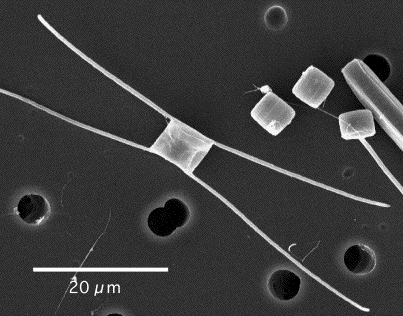
\includegraphics[width=0.5\textwidth]{./figure/Chaetoceros}
                \caption{Microalgae, \textit{Chaetoceros}. Source: sci.sdsu.edu}
                \label{fig:gull}
                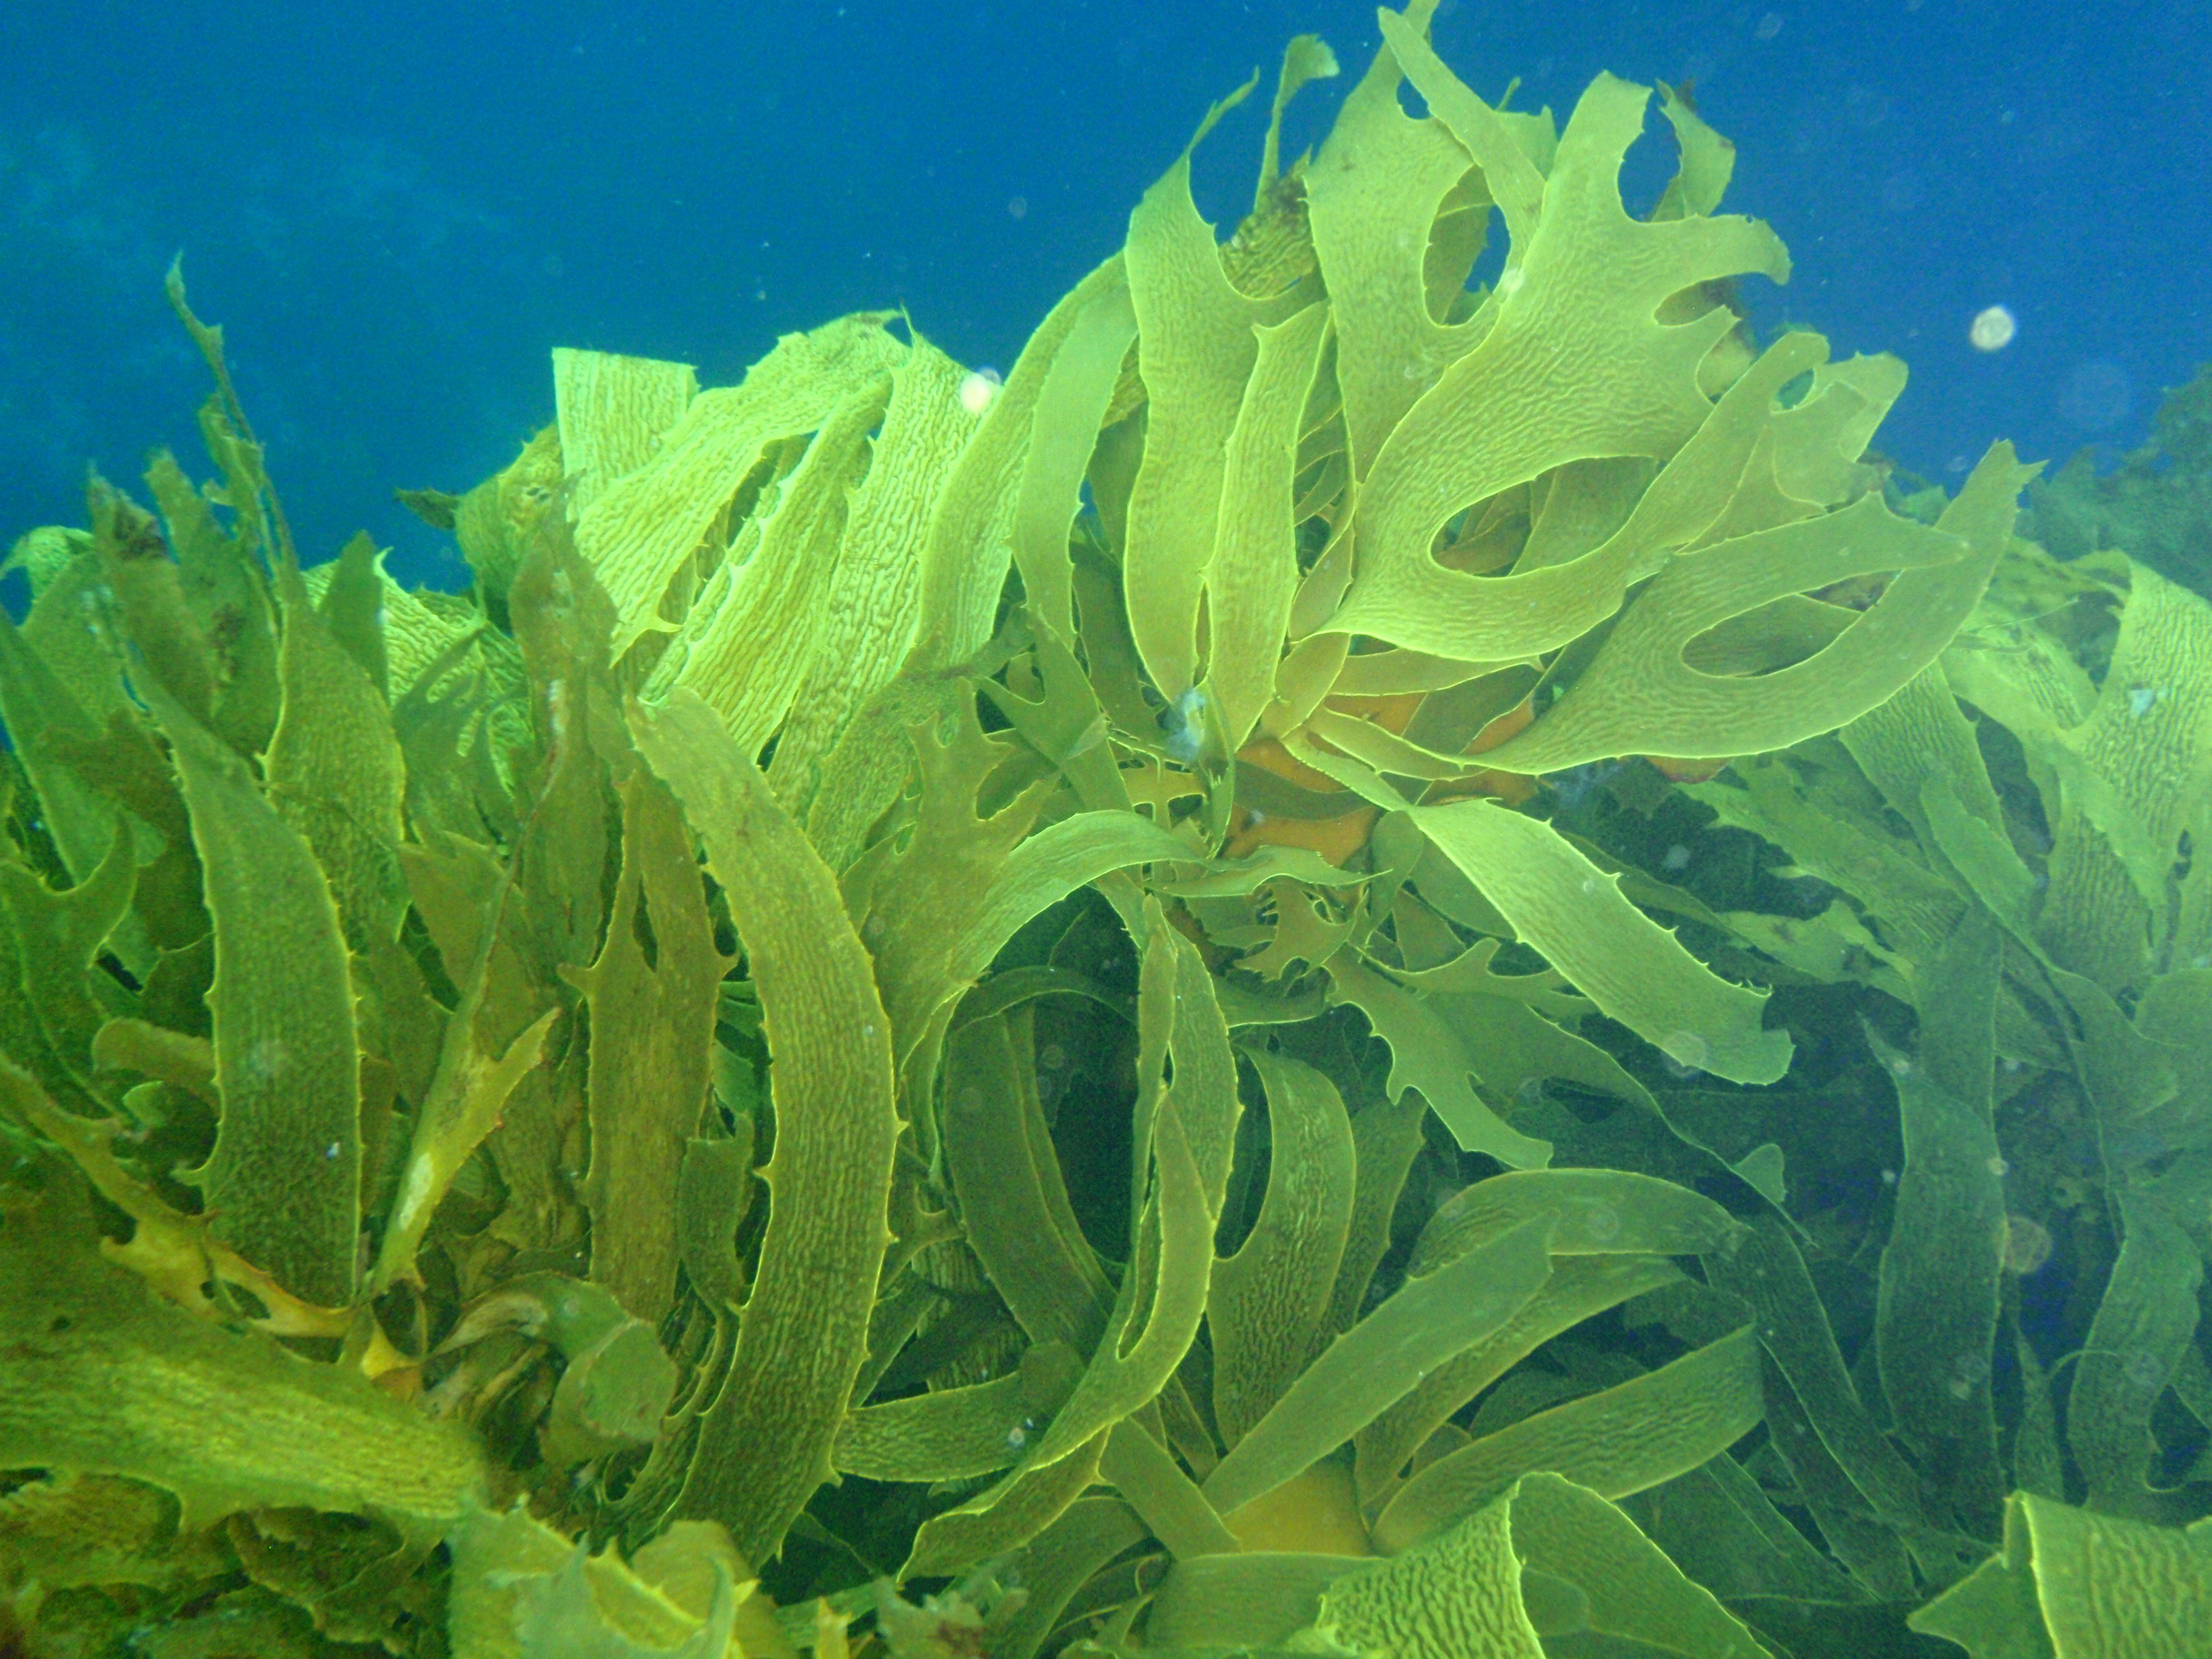
\includegraphics[width=0.5\textwidth]{./figure/Kelp_forest_sciworthy_com}
                \caption{Macroalgae, kelp. Source: Sciworthy.com}
                \label{fig:tiger}
\end{figure}

                \column{.5\textwidth}  
                        \begin{figure}
                                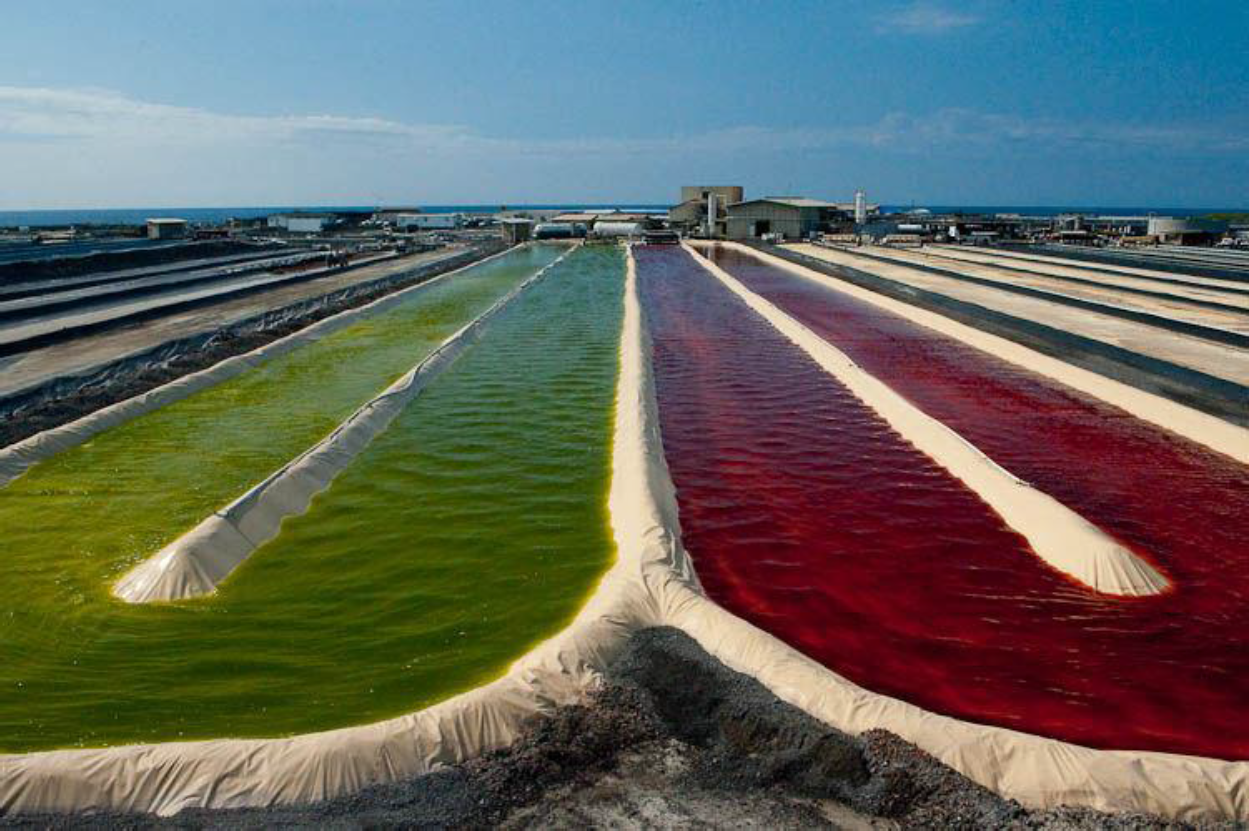
\includegraphics[width=1\textwidth]{./figure/Haematococcus_astaxanthin_Cyanotech.png}
                                \caption{\small{\it Haematococcus} sp. grown for the food supplement astaxanthin. Source: Cyanotech} %$20/4mg, $40/100g, -> $1000+/kg ? %http://web.archive.org/web/20051127023851/http://algatech.com/astax.htm
                        \end{figure}
        \end{columns}

\end{frame}
%%%%%%%%%%%%%%%%%%%%%%%%%%%%
\section{Biofuel}
\begin{frame}{Biofuel}
\begin{itemize}
 \item Renewable resource
    \item High oil content
      \item Need to reduce costs for viability%\cite{menetrez_overview_2012}
      \note[item]{Need to be cost competitive with petroleum based fuels; almost there!}
      \note[item]{Economic model}
      \note[item]{high value/low quantity products such as chemicals,cosmetics, supplements vs. low value/high quantity product such as fuel }
  \item Algal monoculture vs. 'synthetic ecology' of various species%\cite{kazamia_mutualistic_2012}
  \note[item]{Monoculture: pick the single best species, 'Synth. Ecol": resist contamination, different species thrive in different conditions; a benefit for cultures that are subject to varying outdoor conditions}
    \note[item]{some aquaculture species have biofuel potential, same reason they are used as feedstock: lipid content}
  \note[item]{algal monocultures can invite contaminants}%\cite{kazamia_mutualistic_2012}
  \note[item]{Two common growth methods; open ponds and enclosed bioreactors}
  \note[item]{Open ponds are cheaper but require a lot of land, water!!; evaporation. Potential for contamination!}
  \note[item]{Common methods of contamination prevention are fast-growing algal species to overcrowd contaminants, or extreme growth conditions e.g. pH or salinity; Spirulina grown in pH up to 9.0}
  \note[item]{Enclosed reactors resist contamination but are more expensive, require difficult maintenance \& cleaning, conserve water}
  \note[item]{other method: cheap plastic bags}
  \note[item]{Important consideration: light source. Sunlight is free, but less consistent, subjects algae to the elements}
  \note[item]{Electronic light is cooler, more flexible, but costs money! Not viable for low-margin products like biofuel}
  \note[item]{Light penetration through culture as limiting factor in culture growth}
\end{itemize}
\begin{columns}%[t] 
                \column{.5\textwidth}
                        \begin{figure}
                                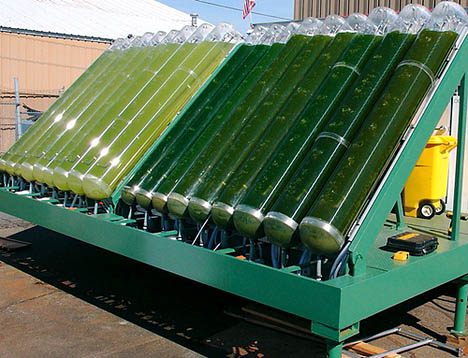
\includegraphics[width=1\textwidth]{./figure/algae-bioreactor_enfo_agt_bme_hu}
                                \caption{Enclosed algal bioreactors. Source: enfo.agt.bme.hu}
                        \end{figure}
                \column{.5\textwidth}  
                        \begin{figure}
                                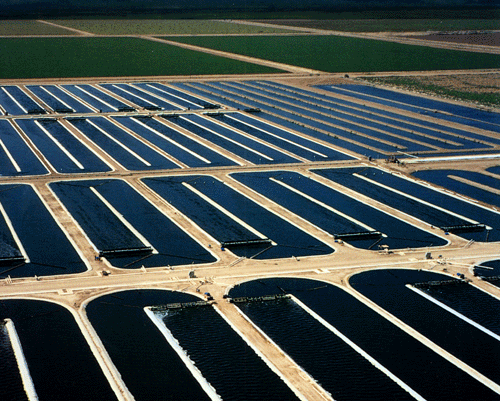
\includegraphics[width=1\textwidth]{./figure/earthrise_farm_pond_ethand_net}
                                \caption{Open raceway ponds. Source: ethand.net}
                        \end{figure}
        \end{columns}
\end{frame}
%%%%%%%%%%%%%%%%%%%%%%%%%%%%
\section{Aquaculture}
\begin{frame}{Aquaculture}
\begin{itemize}
\item Algal feedstock for fin-fish, shrimp, mollusks, etc.
\item Required either directly or indirectly in aquatic animal diets
\note[item]{Algae are primary producers in aquatic food webs, base of all aquatic food chains}
\note[item]{all farmed aquatic animals require algae in their life cycle directly or indirectly} %\cite{wikfors_impact_2001} 
\item Algae culture accounts for up to 40\% of bivalve hatchery costs %\cite{helm_hatchery_2004}
  \note[item]{example: Horn Point Laboratory oyster hatchery, Cambridge, MD}
\item High oil content
  \begin{itemize}
  \item carry over to biofuel
  \end{itemize}
\end{itemize}
\begin{columns}%[t] 
                \column{.5\textwidth}
                        \begin{figure}
                        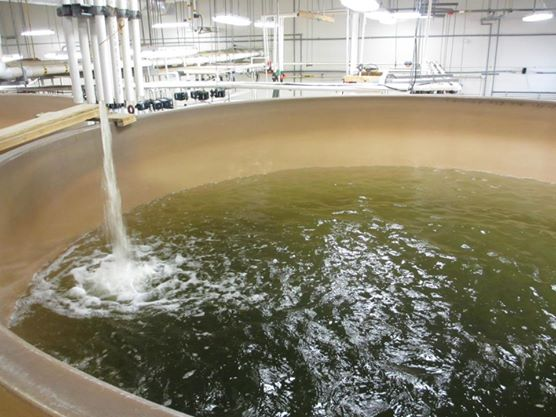
\includegraphics[width=1\textwidth]{./figure/HornPoint2013_Algae_feedstock}
                        \caption{Algal feedstock for oyster larvae. Source: Horn Point Laboratory}
                        \end{figure}
                \column{.5\textwidth}  
                        \begin{figure}
                                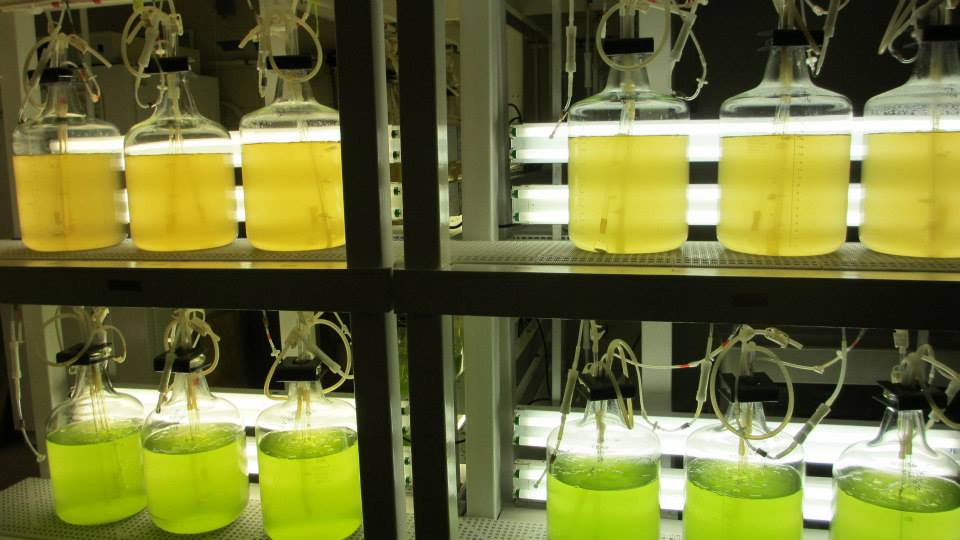
\includegraphics[width=1\textwidth]{./figure/HPL_Experiment_underway.jpg}
                                \caption{Algal starter cultures. Source: Horn Point Laboratory}
                        \end{figure}
        \end{columns}
\end{frame}
%%%%%%%%%%%%%%%%%%%%%%%%%%%%
\section{Algal Species}
\begin{frame}[fragile]{Algal Species Included in the Study}

% latex table generated in R 3.1.1 by xtable 1.7-4 package
% Sun Nov  2 15:32:37 2014
\begin{table}[ht]
\centering
\begin{tabular}{rlll}
  \hline
 & Species & Attributes & Uses \\ 
  \hline
1 & \emph{Tetraselmis chuii} & Chlorophyta - flagellate & Aquaculture feed \\ 
  2 & \emph{Chaetoceros mulleri} & Ochrophyta - diatom & Aquaculture feed \\ 
  3 & \emph{Isochrysis sp.} & Haptophyta - flagellate & Aquaculture feed \\ 
  4 & \emph{Thalassiosira pseudonana} & Ochrophyta - diatom & Aquaculture feed \\ 
  5 & \emph{Nannochloropsis oculatta} & Ochrophyta - flagellate & Potential for biofuel \\ 
   \hline
\end{tabular}
\caption{Algal species used in the study.} 
\label{tab:Algae_Species}
\end{table}

\note[item]{Thalassiosira psuedonana is a model diatom, first to have genome sequenced}
\note[item]{The four aquaculture species together represent a standard diet for oyster larvae}
\begin{columns}[t] %Without t, the columns are centered
                \column{.5\textwidth}
                        \begin{figure}
                                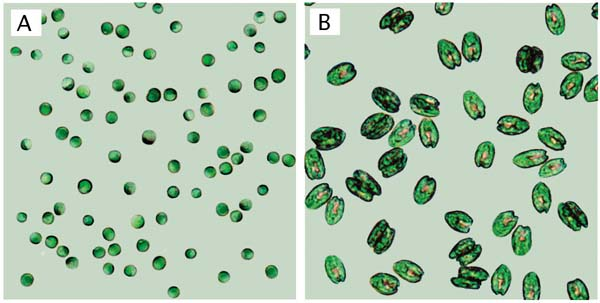
\includegraphics[width=1\textwidth]{./figure/FAO_Isochrysis_Tetraselmis.jpg}
                                \caption{A. {\it Isochrysis} sp.. B. {\it Tetraselmis} sp.. Source: www.fao.org}
                        \end{figure}
                \column{.5\textwidth}  
                        \begin{figure}
                                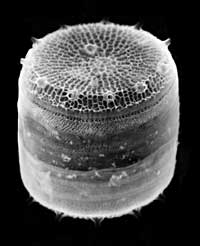
\includegraphics[width=0.4\textwidth]{./figure/Thal_psuedonana.jpg}
                                \caption{{\it Thalassiosira pseudonana} SEM micrograph. Source: www.jgi.doe.gov}
                        \end{figure}
        \end{columns}

\end{frame}
%%%%%%%%%%%%%%%%%%%%%%%%%%%%
\begin{frame}{Travel}
\begin{itemize}
% \item Learn more about algae and aquaculture
\item Horn Point Laboratories, Cambridge, MD
\note[item]{provided guidance, aquaculture algal samples}
\item UTEX Culture Collection of Algae, University of Texas, Austin, TX
\note[item]{attended 2 day seminar on microalgal culture growth and management, provided algal sample}
\end{itemize}
\begin{columns}%[t] %Without t, the columns are centered
                \column{.5\textwidth}
                        \begin{figure}
                                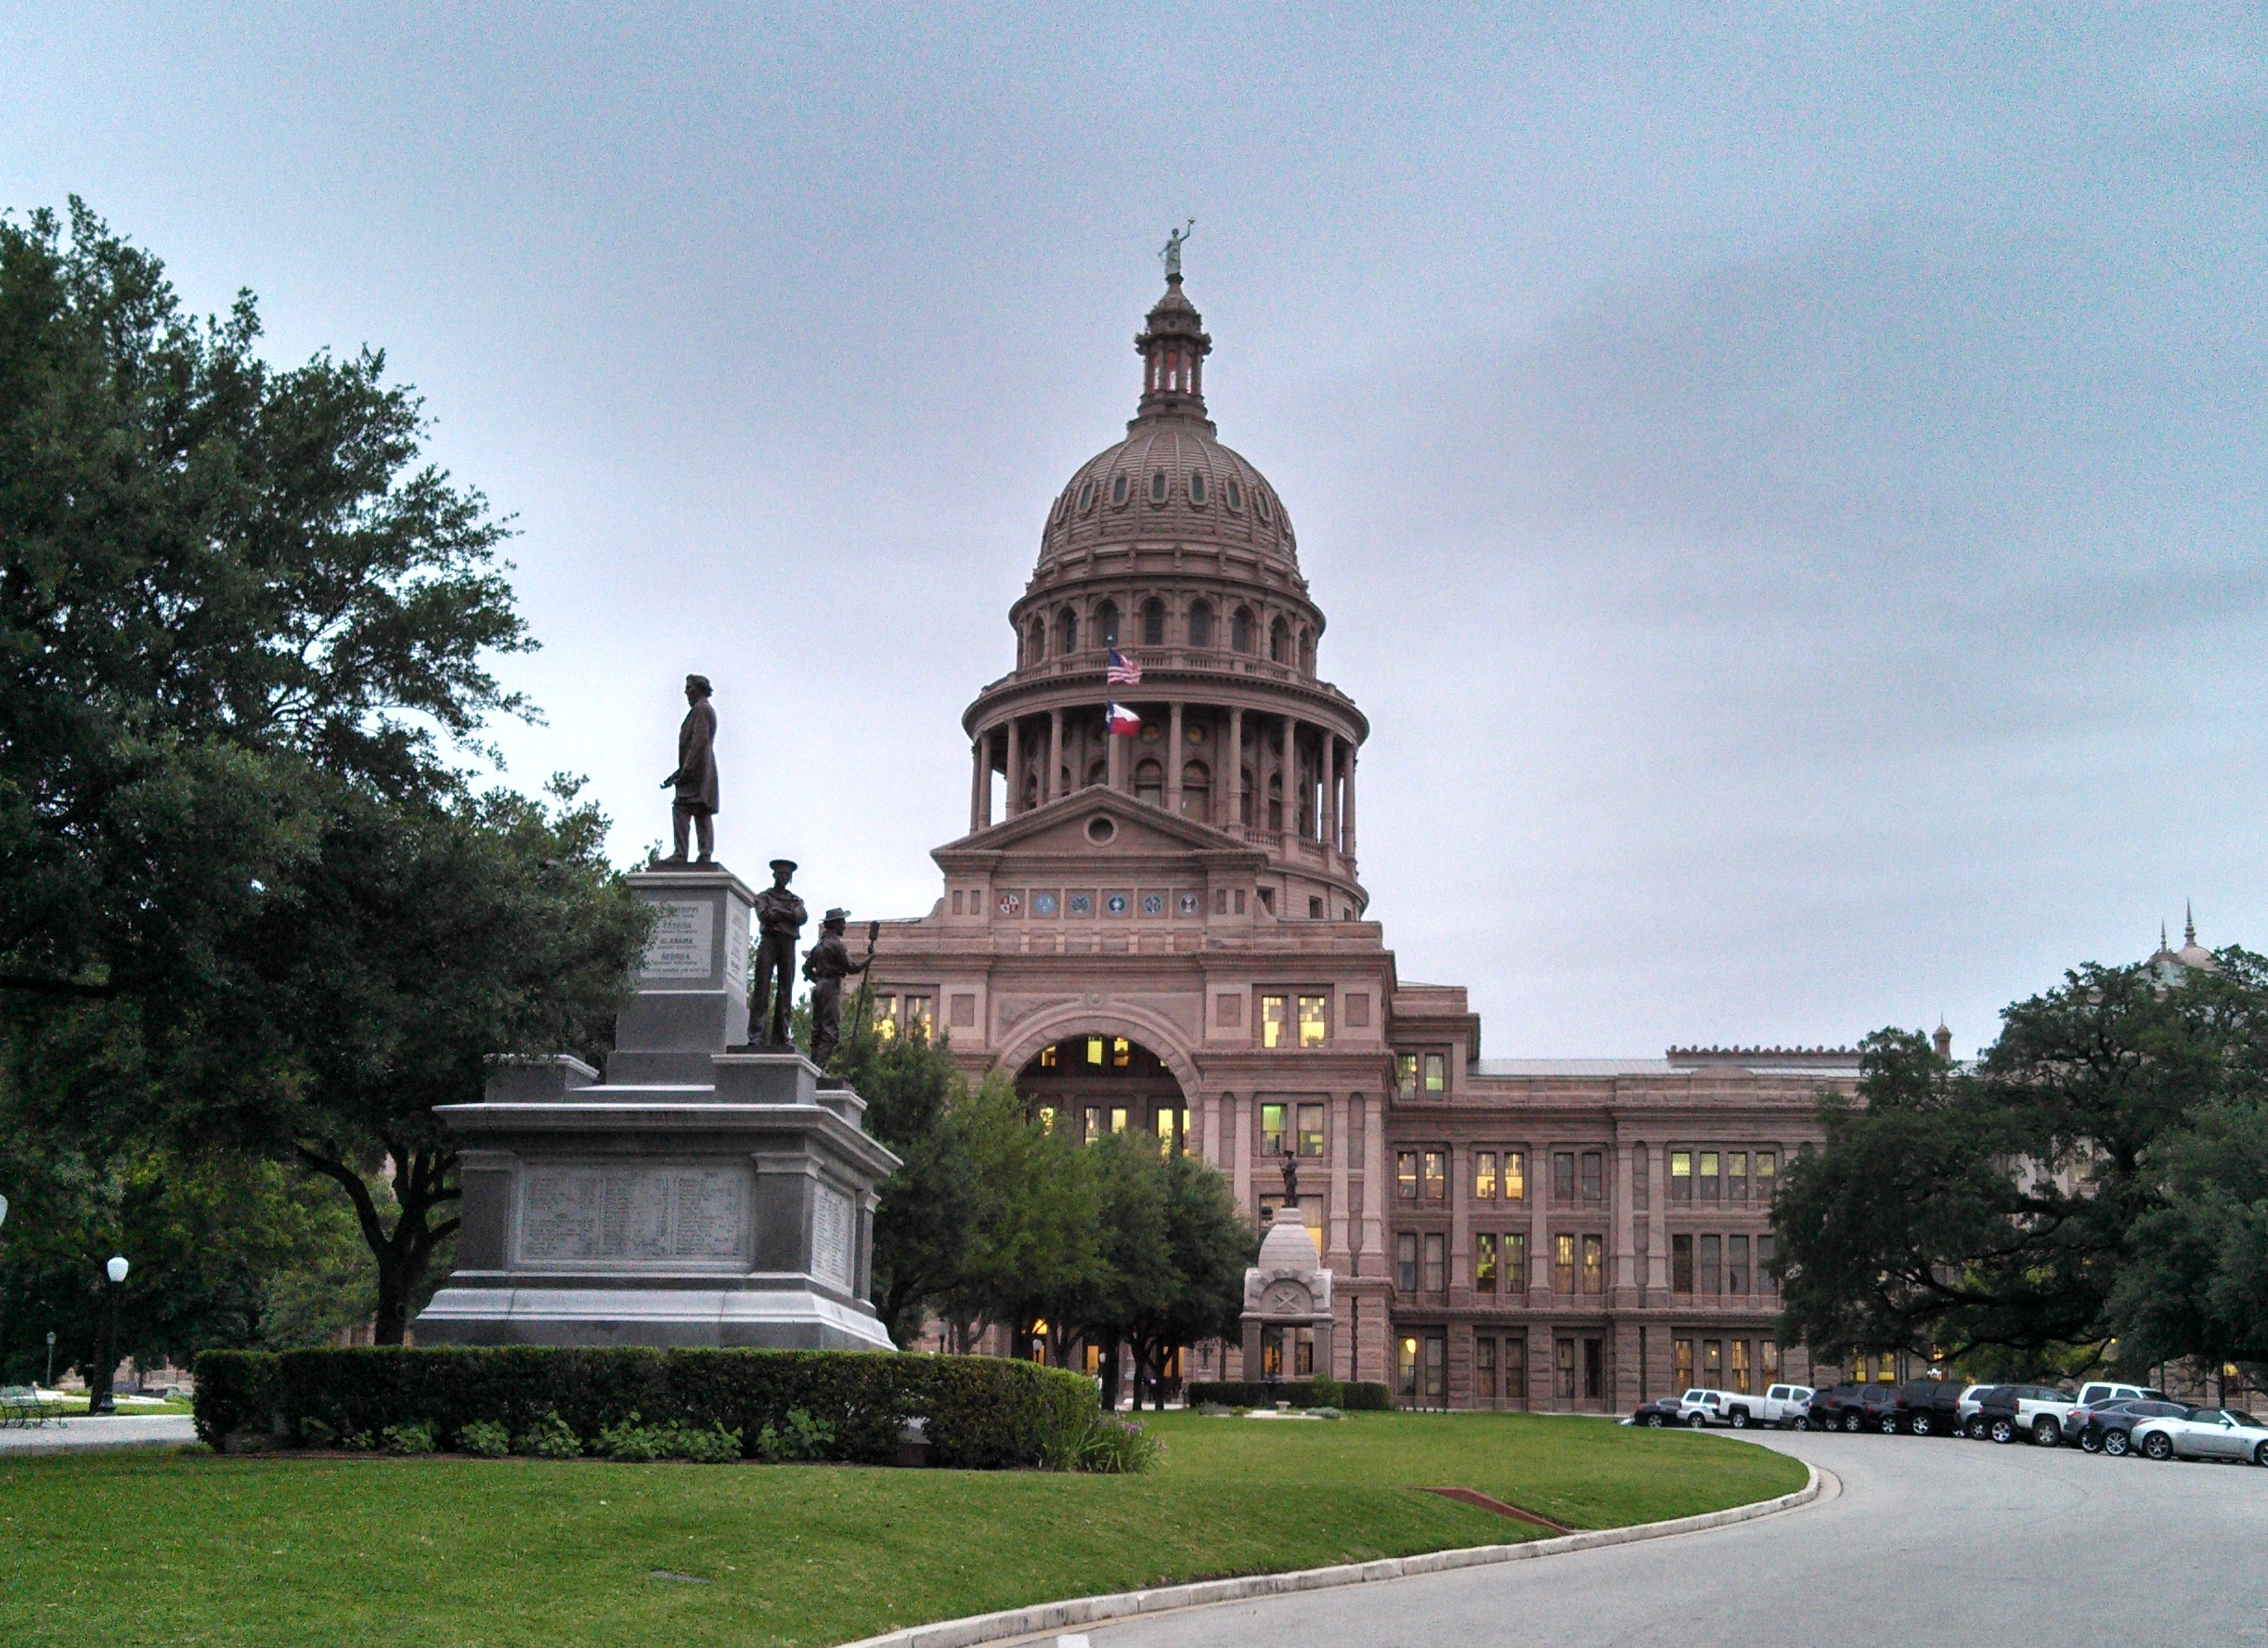
\includegraphics[width=0.6\textwidth]{./figure/UTEX_Austin_TX_capitol}
                                \caption{Capitol building at Austin, Texas.}
                        \end{figure}
                        \begin{figure}
                                \includegraphics[width=0.6\textwidth]{./figure/Texas_cycad}
                                \caption{Austin: Home to massive cycads}

                        \end{figure}
                \column{.5\textwidth}  
                        \begin{figure}
                                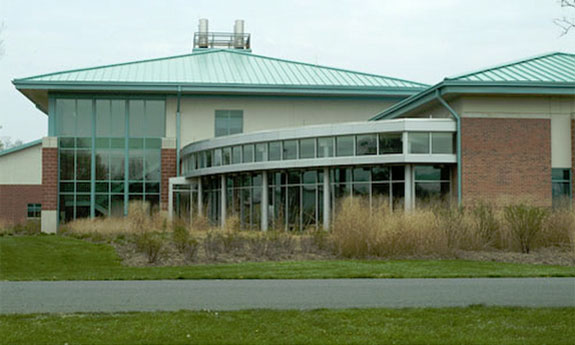
\includegraphics[width=1\textwidth]{./figure/HornPointLab}
                                \caption{Horn Point Aquaculture and Restoration Ecology Laboratory. Source: http://hatchery.hpl.umces.edu/}
                        \end{figure}
        \end{columns}
\end{frame}
%%%%%%%%%%%%%%%%%%%%%%%%%
\section{PPFM}
\begin{frame}{Pink Pigmented Facultatively Methylotrophic Bacteria}
\begin{itemize}
\item PPFM, genus {\it Methylobacterium}
\note[item]{rod shaped, gram negative bacteria}
\item Ubiquitous plant symbionts
  \note[item]{found on every plant surface tested}
  \note[item]{especially on actively growing plant surfaces; MeOH as waste product from plant cell wall breakdown during growth}
\item Able to metabolize Methanol
  \note[item]{remember, facultatively =  can metabolize MeOH in addition to regular C sources}
\item Stimulate plant growth, enhance seed germination, produce plant growth regulators %\cite{holland_methylobacterium_2002}
\item Can be isolated from water, algae samples
\end{itemize}

\begin{figure}
    \centering
    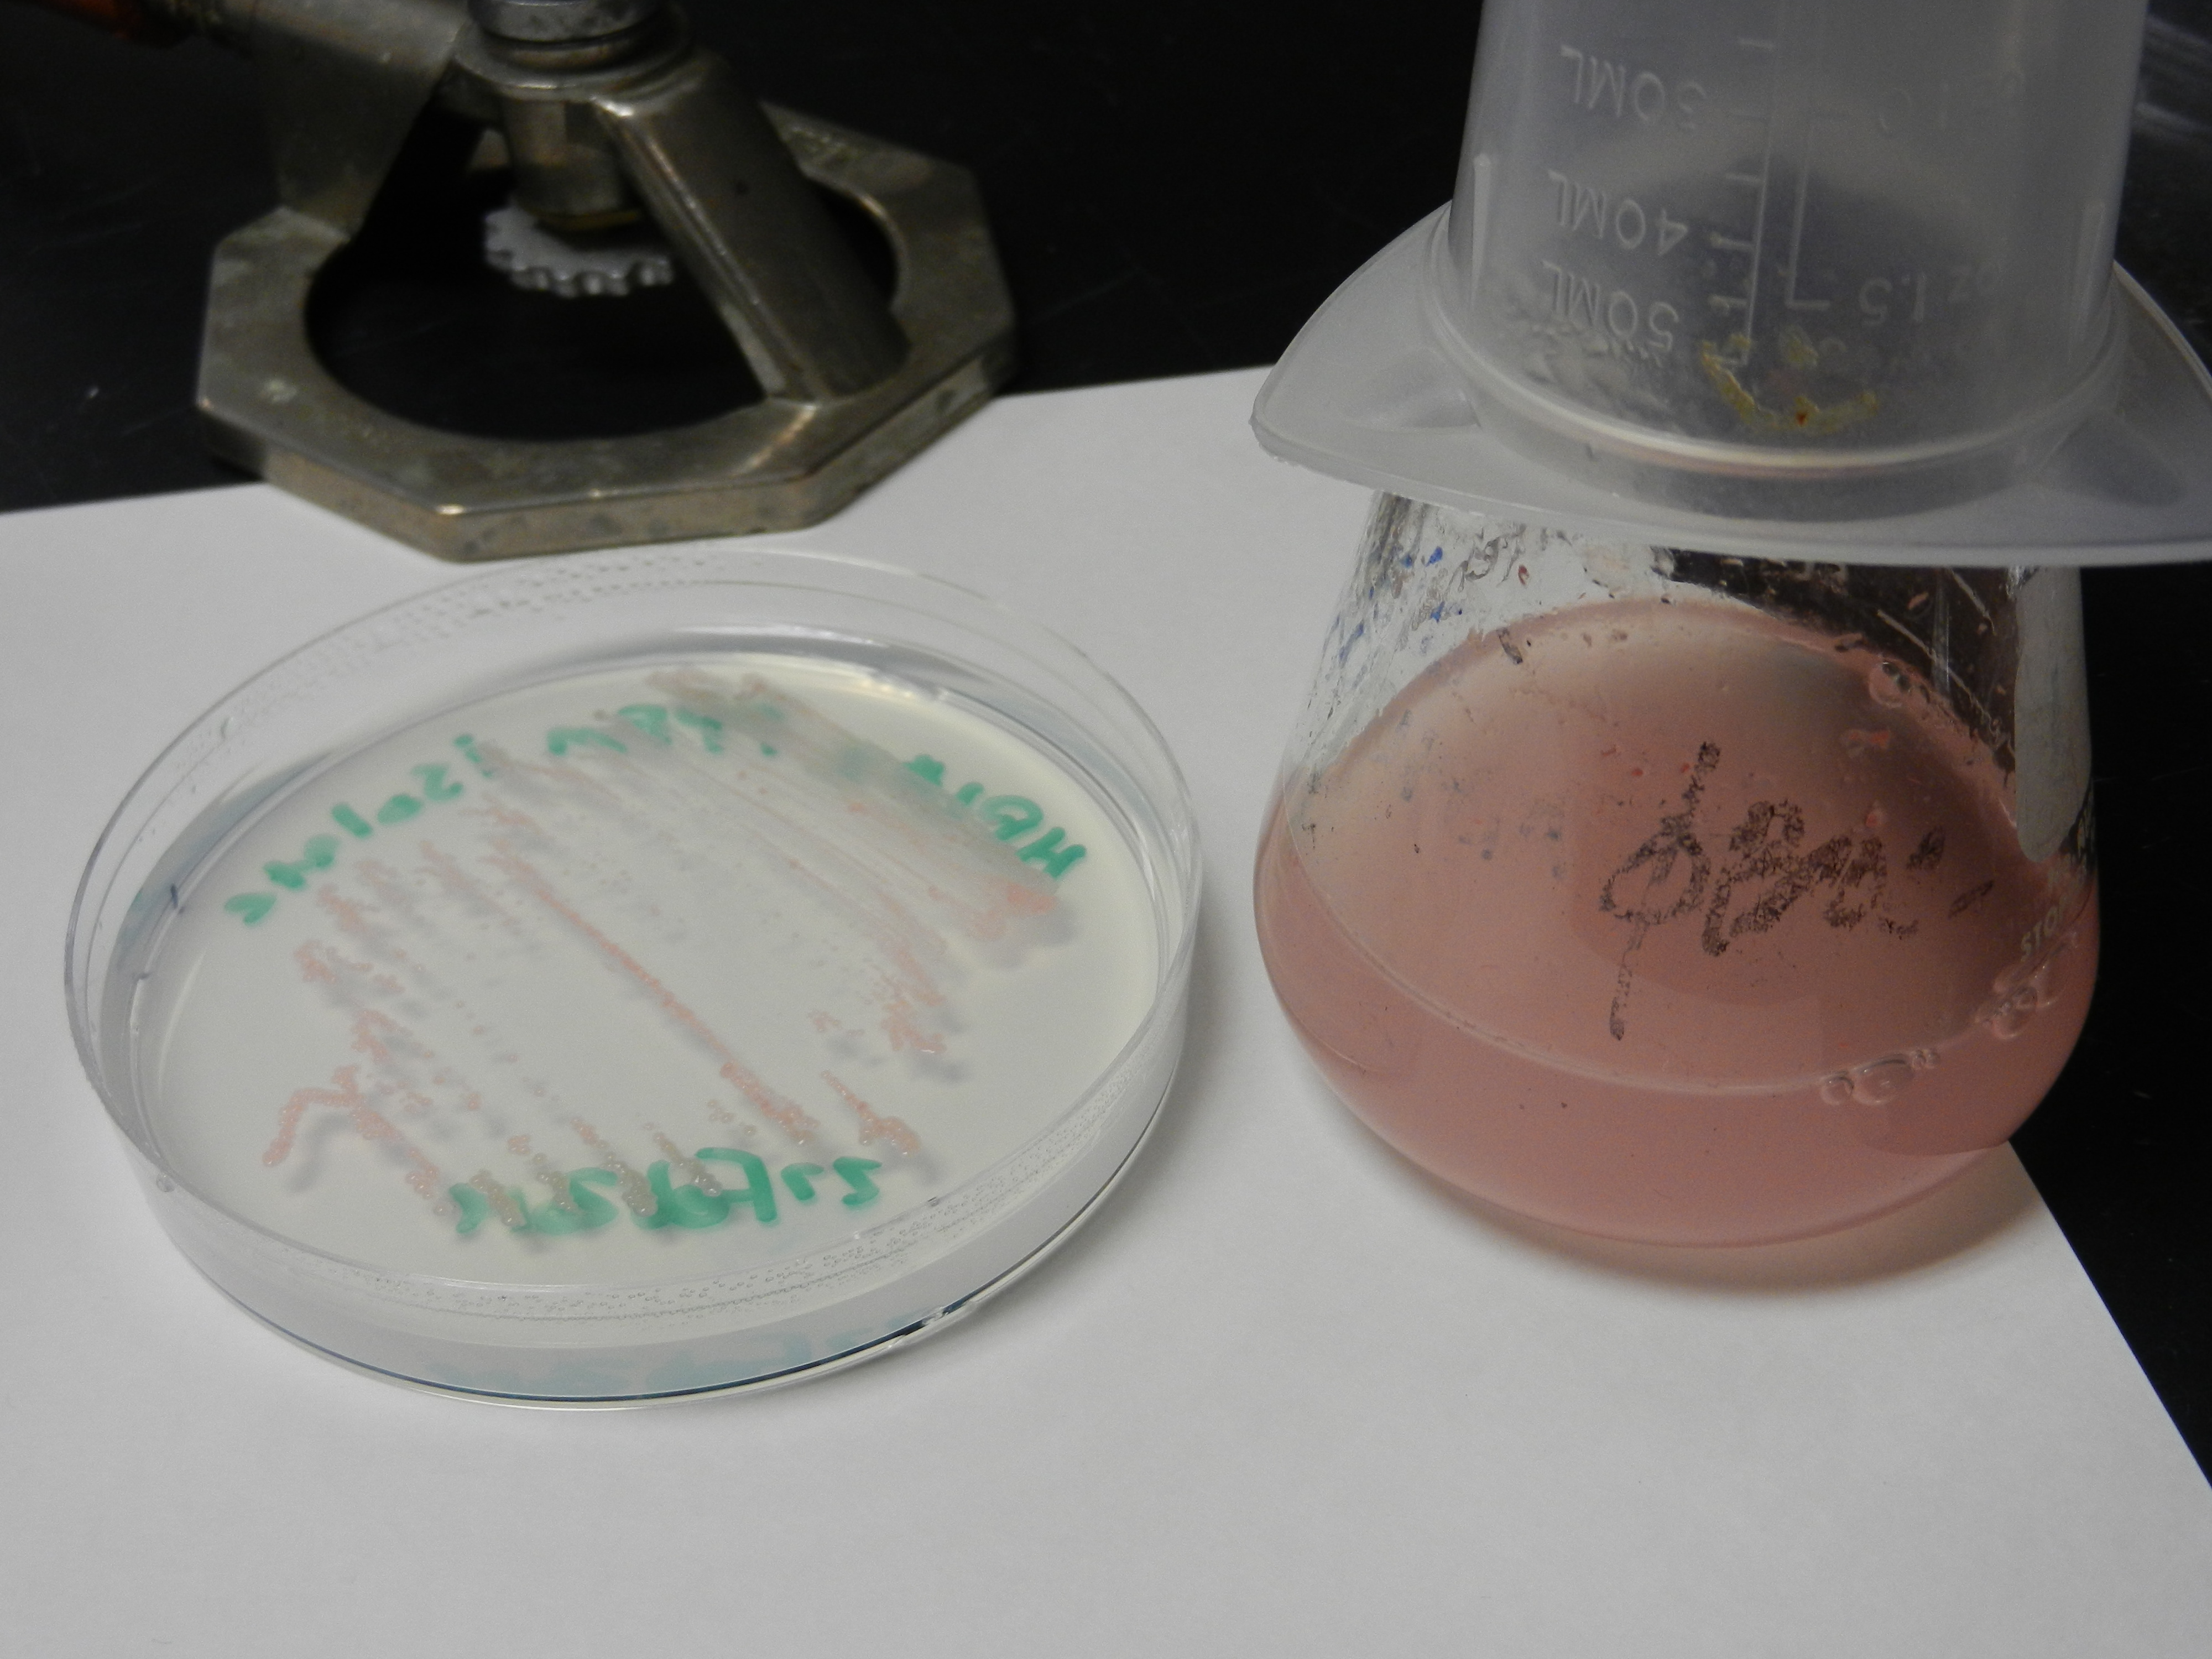
\includegraphics[width=0.5\textwidth]{./figure/PPFM_Cultures.JPG}
    \caption{Solid and liquid PPFM cultures}
    \label{}
\end{figure}

\end{frame}
%%%%%%%%%%%%%%%%%%%%%%%%%%%%
\begin{frame}{Why PPFM's?}
\begin{itemize}
\item Avoid genetic modification of algae
\item Inexpensive
\item Naturally occurring
\item Past research suggests potential
\end{itemize}

\begin{figure}%[b]
%     \centering
    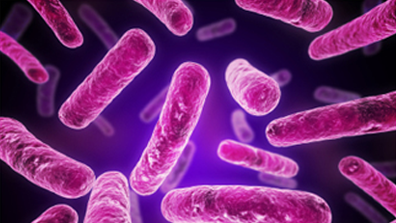
\includegraphics[width=0.5\textwidth]{./figure/ppfm_newleafsym_com}
    \caption{Rendering of PPFM. Source: newleafsym.com}
\end{figure}

\end{frame}
%%%%%%%%%%%%%%%%%
\section{Past Research}
\begin{frame}{Past Research}
\begin{itemize}
\item Vitamin B12 overproducing strain of PPFM isolated
\note[item]{Many species of microalgae are B12 auxotrophs}
\item Patented bacterization technology for plants
  \begin{itemize}
  \item NewLeaf Symbiotics, LLC.
  \end{itemize}
\item PPFM supplementation enhanced algal growth in {\it Chlamydomonas} (unpublished; Chuck Davis, 2010)
  \note[item]{also in Neochloris oleoabundans, lipid concentration study}
  \note[item]{different ratios of PPFM:algae tested, 5:1 showed good results}
\end{itemize}

\begin{figure}
    \centering
    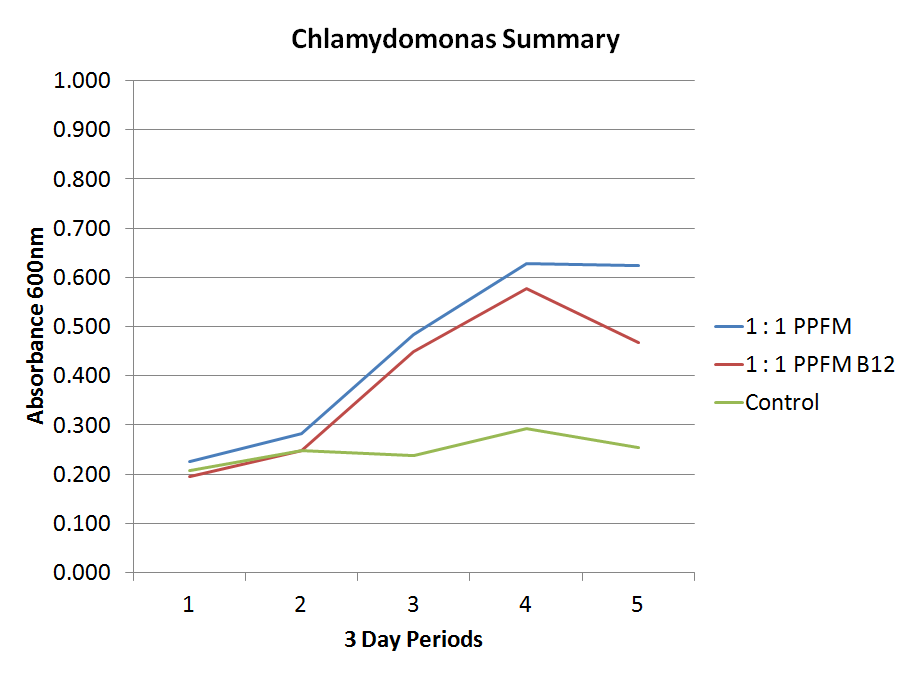
\includegraphics[width=0.6\textwidth]{./figure/Chlamydomonas_summary}
    \label{}
\end{figure}
\end{frame}
% %%%%%%%%%%%%%%%%
\section{Goals}
\begin{frame}{Research Goals \& Hypotheses}
\begin{itemize}
\item Supplementation with PPFM will benefit microalgae 
\end{itemize}
%~
\begin{itemize}
  \item Identify PPFM strains
  \item Test for increased algal growth rate with PPFM supplementation
  \item Test for increased algal nutritional qualities with PPFM supplementation
\end{itemize}

% \begin{columns}[t] 
%  \column{1\textwidth}

% \end{columns}
\end{frame}
%%%%%%%%%%%%%%%%%%%%%%%%%%%%
\section{Identify PPFM}
\begin{frame}{PPFM Isolation \& Identification}
 \begin{itemize}
 \item Plate algal sample on AMS + 0.5\% MeOH agar
     \note[item]{AMS ammonium mineral salts, MeOH is the only carbon source}
 \item 16s rDNA amplification \& sequencing
      \note[item]{some strains used in lab have not been formally identified to species level}

    \end{itemize}
\begin{figure}
    \centering
    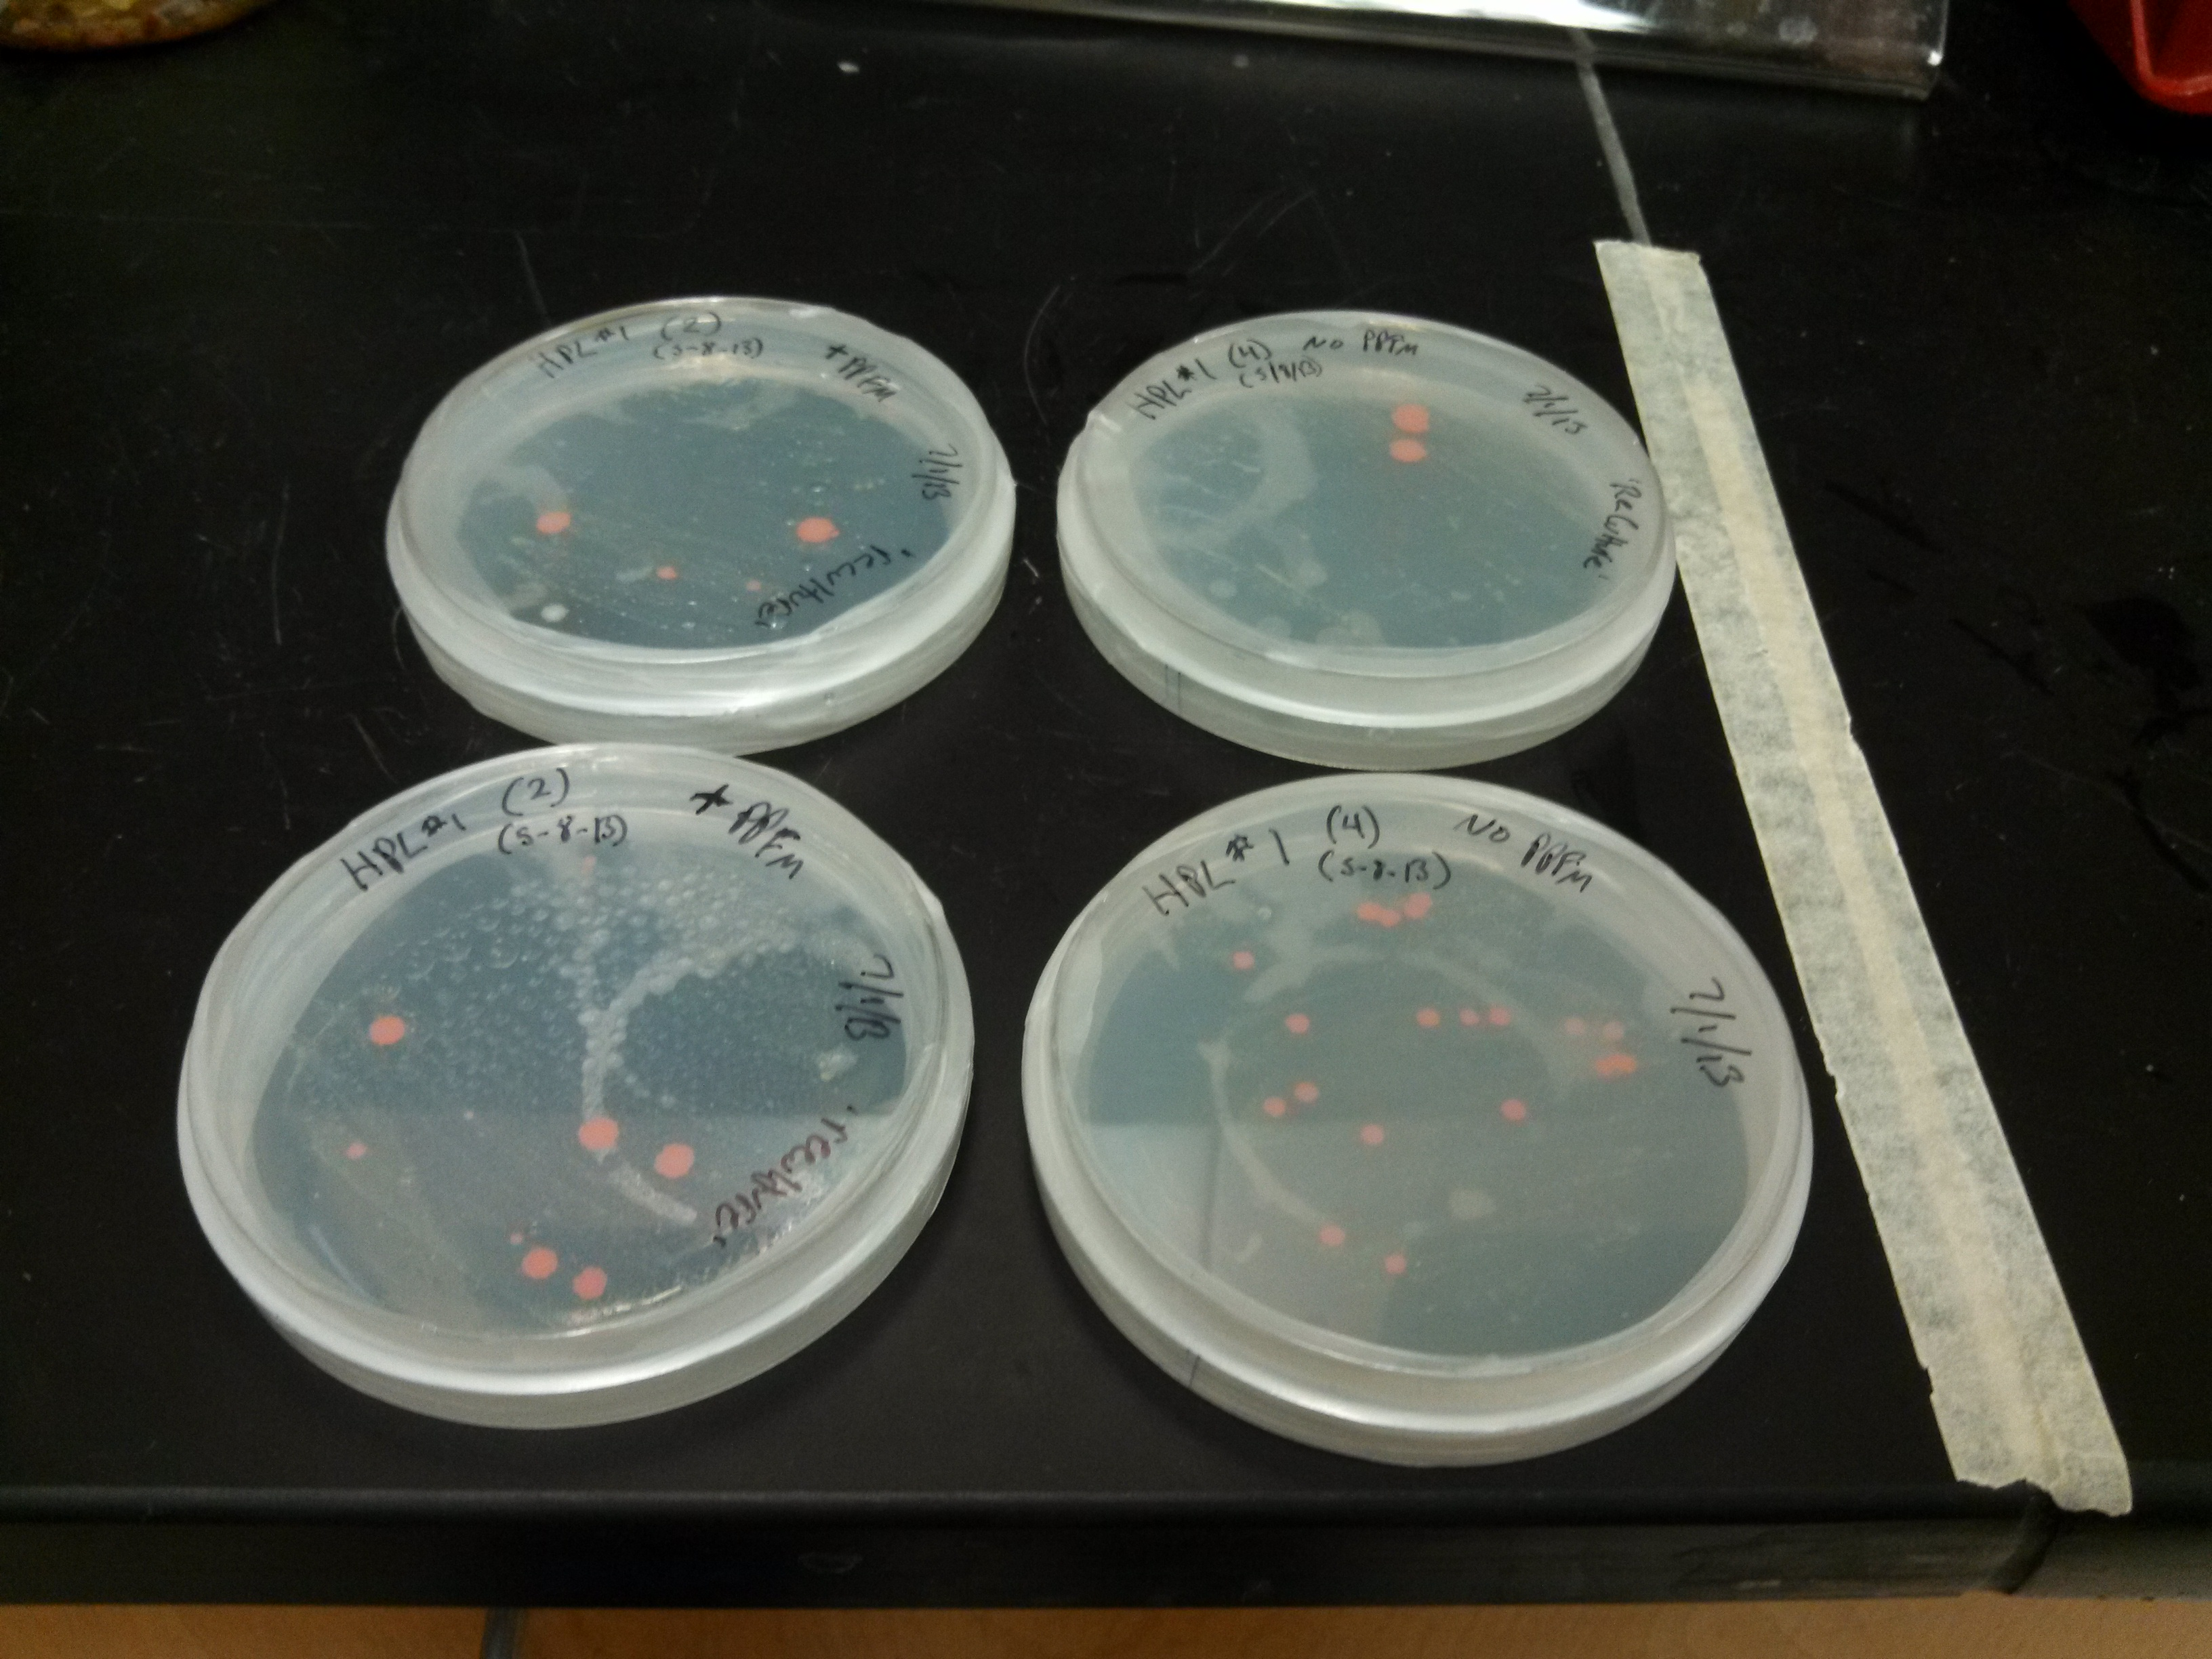
\includegraphics[width=0.6\textwidth]{./figure/Algae_PPFM_isolation}%[width=0.3\textwidth]
    \caption{PPFM colonies forming on plated algae}
\end{figure}
\end{frame}
%%%%%%%%%%%%%%%%%%%%
\section{Algal Growth}
\begin{frame}{Algal Growth Analysis}

\begin{itemize}
\item Correlate \textbf{\textcolor{green}{chlorophyll} \textcolor{purple}{auto}\textcolor{red}{fluorescence}} with cell density
  \note[item]{Explain how fluorescence, autofluorescence works!!}
  \note[item]{Fluorescence Excitation: 436nm (near-UV), Emission: 680nm (red)}
  \note[item]{used fancy sidearm flasks, had to tilt machine to prevent spilling}
  \note[item]{had to take readings at night! machine lid open}
  \note[item]{Dr. Erickson's Spectra Max i3 plate reader also used}
\item Algae grown \(\pm\) PPFM, vitamin B12 over-producing PPFM
\item 'Day 7' critical factor, replicate industrial media and conditions
  \note[item]{looking for economically important aspects}
  \note[item]{trying to mirror 'real world' industrial conditions, using standard F2 media, fluorometer}
  \end{itemize}
\begin{columns}
                \column{.5\textwidth}
                        \begin{figure}
                                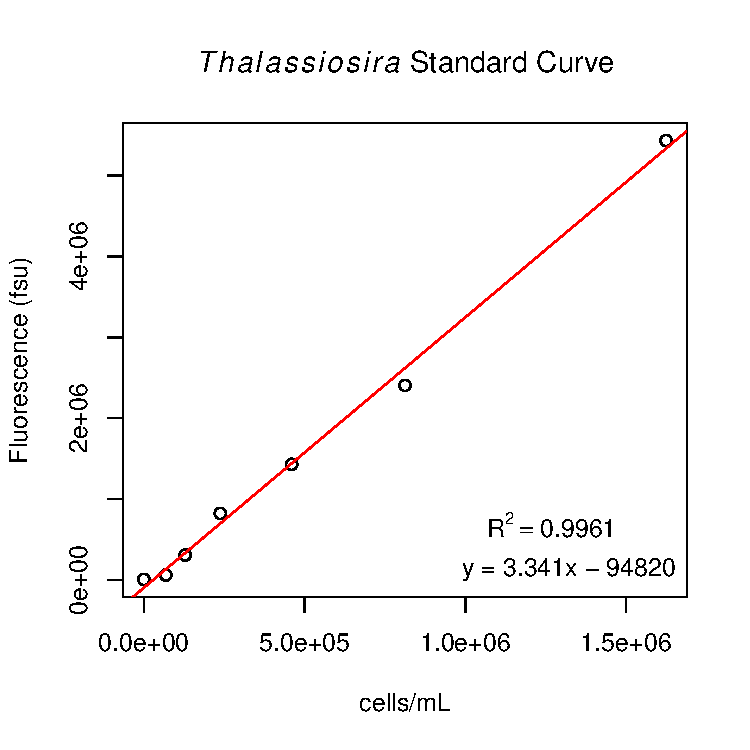
\includegraphics[width=1\textwidth]{./figure/ExpM_MiniThal_StdCurve1_unlabeled2}
                        \end{figure}
                \column{.5\textwidth}  
                        \begin{figure}
                                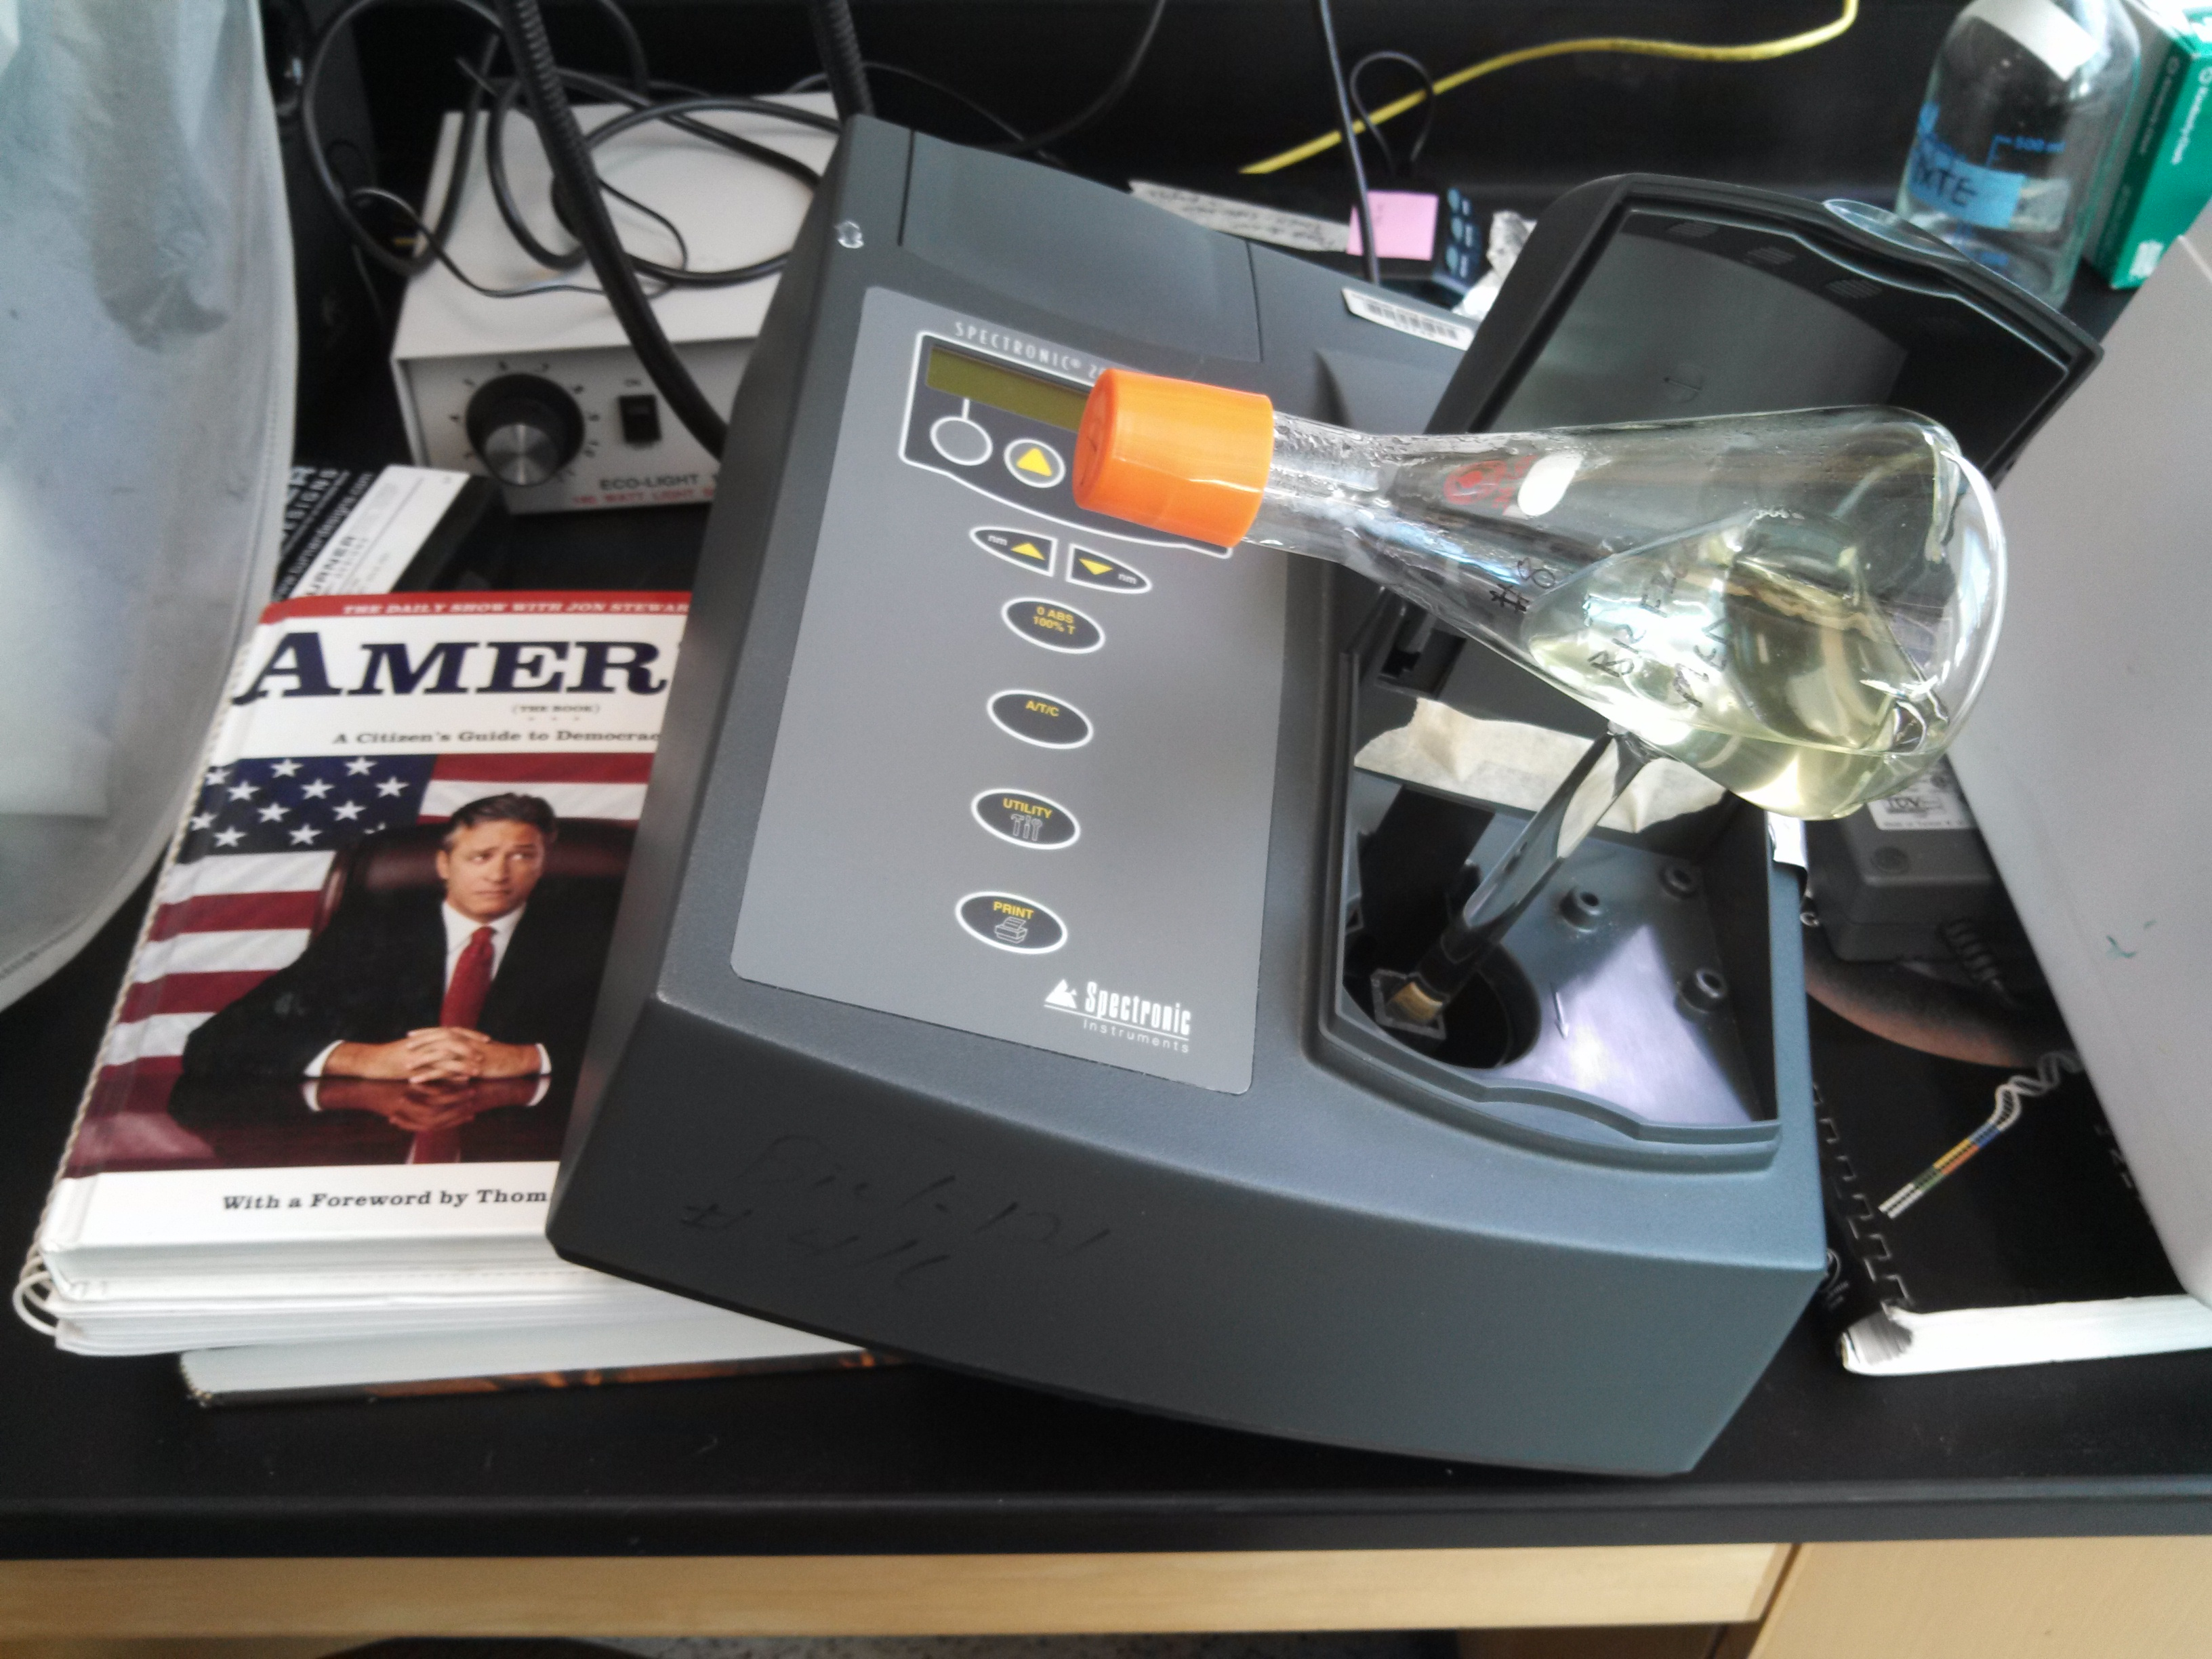
\includegraphics[width=1\textwidth]{./figure/AlgaeReadingSpec.jpg}
                                \caption{Research supported by Jon Stewart}
                        \end{figure}
        \end{columns}
\end{frame}
%%%%%%%%%%%%%%
% \section{Thalassiosira}
\begin{frame}{Results:{\it Thalassiosira}}
\note[item]{No difference seen here...}
\begin{columns}[t] %Without t, the columns are centered
                \column{.5\textwidth}
                \begin{figure}
                                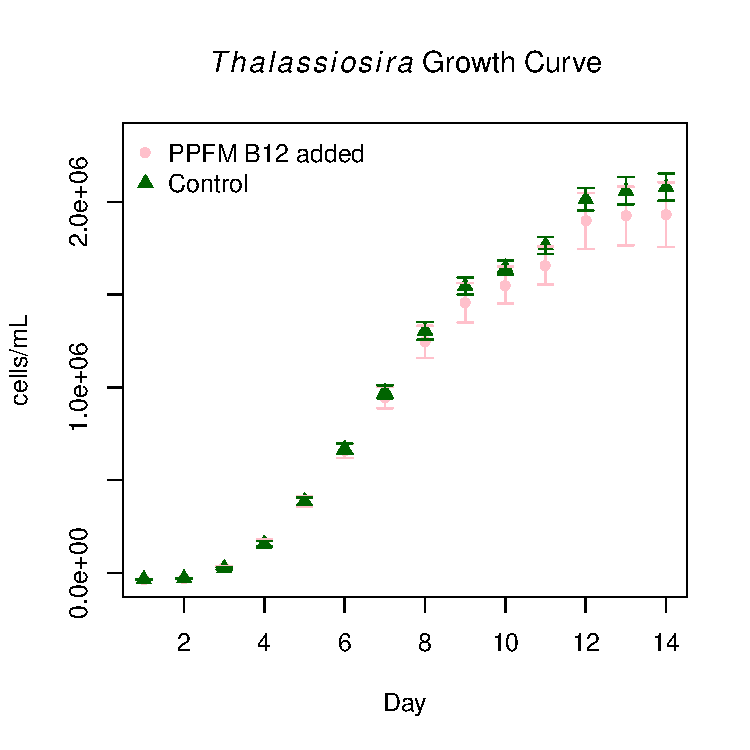
\includegraphics[width=1\textwidth]{./figure/Thalassiosira_Scatter_with_SD_errors.pdf}
                                \end{figure}
                                \column{.5\textwidth}
                                \begin{figure}
                                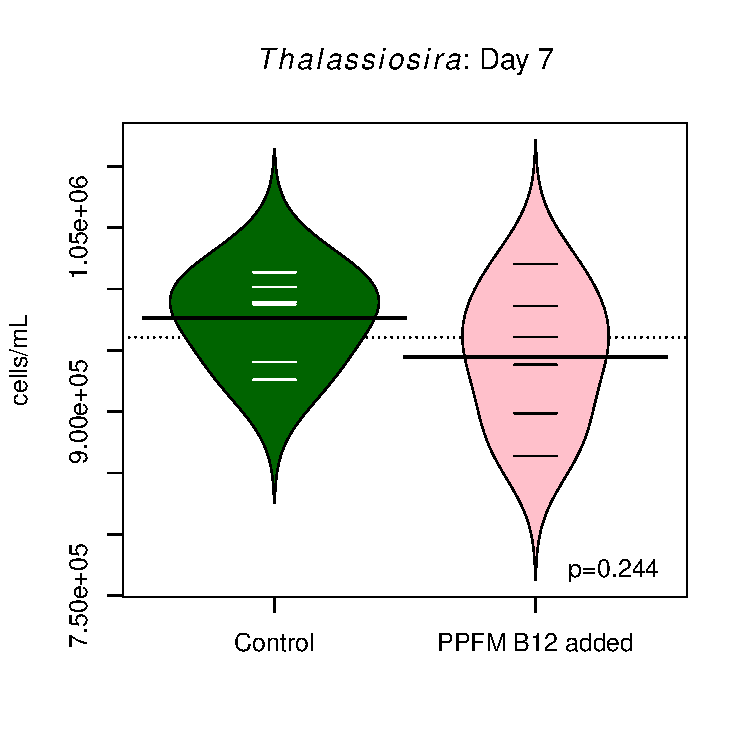
\includegraphics[width=1\textwidth]{./figure/Thalassiosira_beanopplot.pdf}
                                \end{figure}
        \end{columns}

\end{frame}
%%%$%%%%%%%
\begin{frame}{Results:{\it Tetraselmis}}
\note[item]{Algae supplemented with PPFM at 5:1 ratio because past studies showed good results with this}
\note[item]{PPFM B12 selected due to perceived potential; previous IP, known algal B12 auxotrophy}
\note[item]{Standard algae media: F/2, includes vitamin B12! Hatcheries use concentrated F/2 with B12 already included!}
\note[item]{Want to show a benefit from adding the PPFM B12 in an industrial setting}
\note[item]{Tetraselmis showed no difference in growth}
\begin{columns}[t] %Without t, the columns are centered
                \column{.5\textwidth}
                \begin{figure}
                                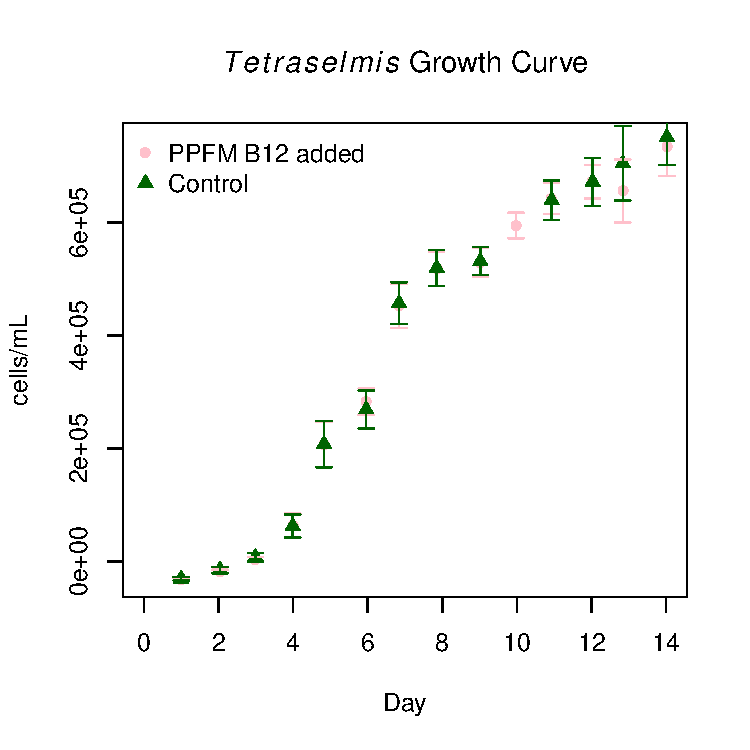
\includegraphics[width=1\textwidth]{./figure/Tetraselmis_Scatter_with_SD_errors.pdf}
                                \end{figure}
                        \column{.5\textwidth}
                        \begin{figure}
                                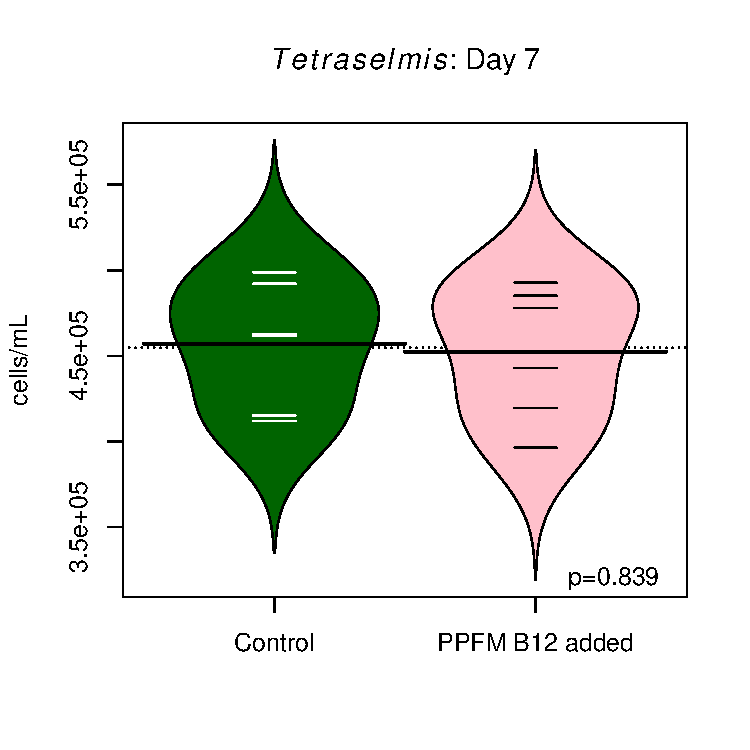
\includegraphics[width=1\textwidth]{./figure/Tetraselmis_beanplot.pdf}
                                \end{figure}
                                \end{columns}
\end{frame}
%%%%%%%%%%%%%%%%%%%%%%%%%
% \section{Mixed Culture}
\begin{frame}{Results: Mixed Culture}
\begin{itemize}
\item Four aquaculture species grown together
\note[item]{We have a statistically significant difference! And by Day 7 too}
\begin{itemize}
\item \textit{Tetraselmis, Thalassiosira, Isochrysis, Chaetoceros}
\end{itemize}
\end{itemize}
\begin{columns}[t] %Without t, the columns are centered
                \column{.5\textwidth}
                \begin{figure}
                                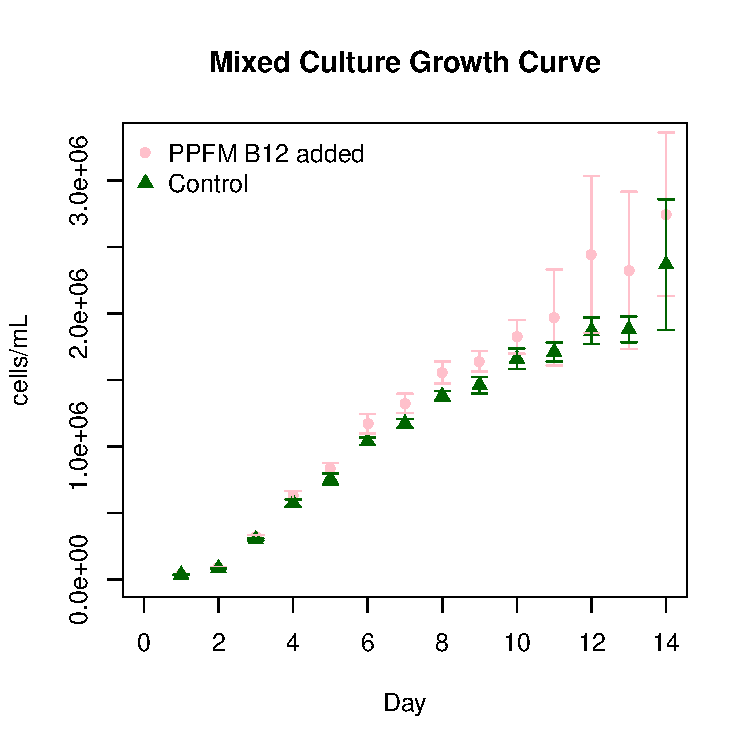
\includegraphics[width=1\textwidth]{./figure/MixedCulture_Scatter_with_SD_errors.pdf}
                                \end{figure}
                                \column{.5\textwidth}
                                \begin{figure}
                                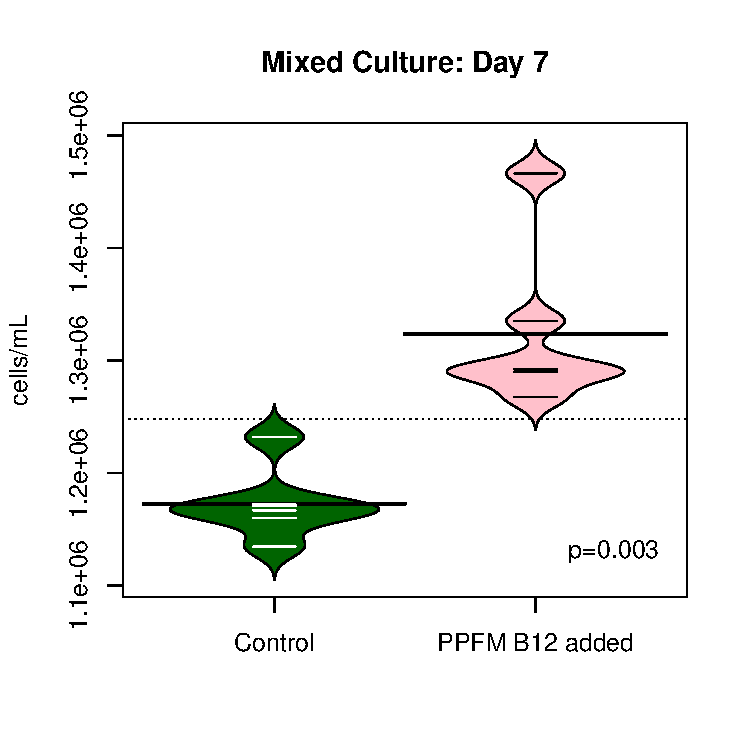
\includegraphics[width=1\textwidth]{./figure/MixedCulture_beanopplot.pdf}
                                \end{figure}
        \end{columns}
\end{frame}
%%%%%%%%%%%%%%
\begin{frame}{Results: B12 Deficient Media}
\note[item]{issues: Vitamin B12 possible contamination from 'dirty' glassware, requires acid wash}
\note[item]{issues: Contamination in B12 deficient media flasks}
\note[item]{Want to show effects of PPFM in B12 deficient and full media}
\note[item]{ExpC: contains PPFM Broc}
\note[item]{ExpD: contains Deficient Media + PPFM B12}
\note[item]{ExpC was run with standard flasks, removing samples for Fluor and Spec analysis}
\note[item]{ExpC Defic. Control had growth outlier, potential for B12 contamination from previous use of flasks}
\note[item]{ExpD Defic. Control had contamination, had to remove one flask for final n=2, but still potential for contamination in remaining flasks}

\begin{columns}[t]
                \column{.5\textwidth}
                \begin{figure}
    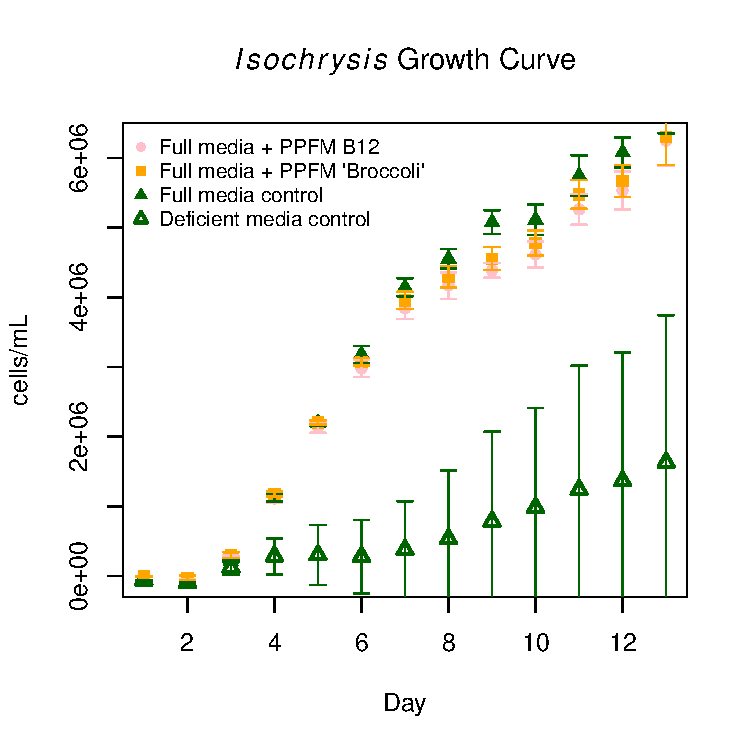
\includegraphics[width=1\textwidth]{./figure/ExpC_GrowthCurve1_unlabeled.pdf}
                                \end{figure}
                                \column{.5\textwidth}
                                \begin{figure}
    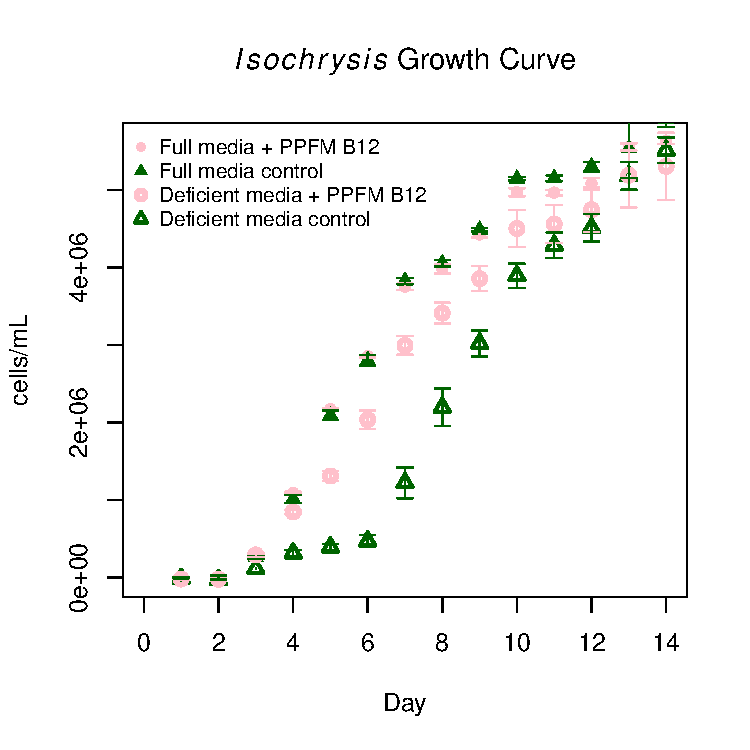
\includegraphics[width=1\textwidth]{./figure/ExpD_GrowthCurve1_unlabeled.pdf}
                                \end{figure}
        \end{columns}
\end{frame}
%%%%%%%%%%%%%%
\begin{frame}{Results: B12 Deficient Media cont.}
\note[item]{Small Volume: algae grown in 15mL Falcon Tubes, n=5}
\note[item]{Measurements taken on 2uL sample, in Spectra Max i3 plate reader}
\note[item]{Fluorescence Excitation: 436nm, Emission: 680nm}

% \begin{figure}
%     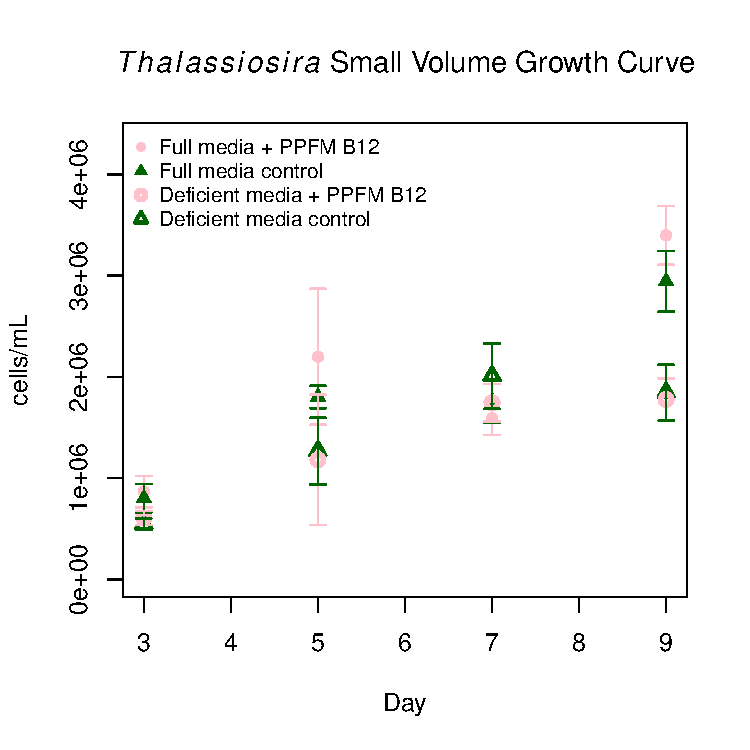
\includegraphics[width=0.6\textwidth]{./figure/ExpM_GrowthCurve2_unlabeled.pdf}
%                                 \end{figure}
                                
\begin{columns}%[t] 
                \column{.5\textwidth}
                        \begin{figure}
                                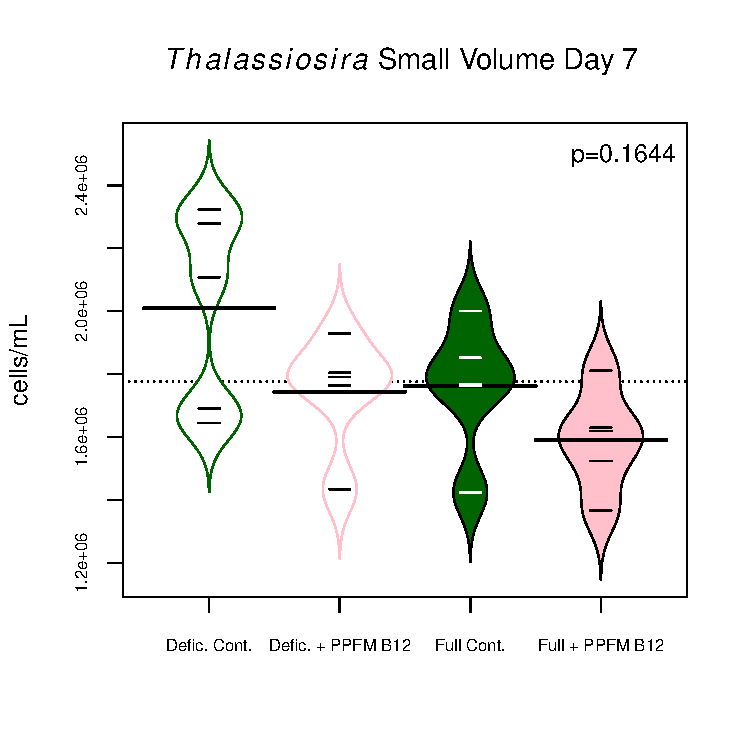
\includegraphics[width=0.7\textwidth]{./figure/ExpM_MiniThal_beanplot_cells_7_unlabeled}
                        \end{figure}
                        \begin{figure}
                                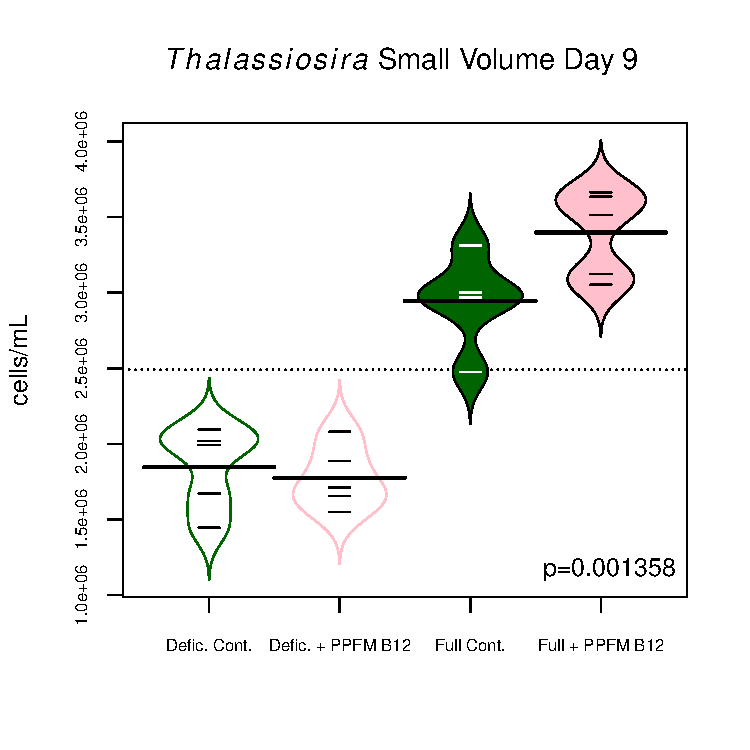
\includegraphics[width=0.7\textwidth]{./figure/ExpM_MiniThal_beanplot_cells_9_unlabeled}
                        \end{figure}
                \column{.5\textwidth}  
                        \begin{figure}
                                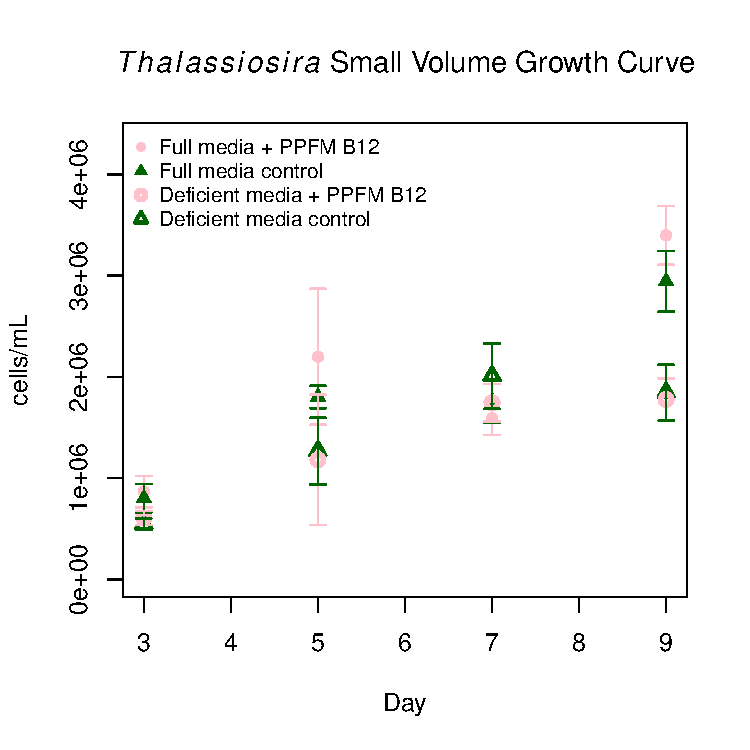
\includegraphics[width=1\textwidth]{./figure/ExpM_GrowthCurve2_unlabeled}
                        \end{figure}
                                                \end{columns}

                        \end{frame}
                        
%%%%%%%%%%%%%%%
\begin{frame}{PPFM Ratio}
\begin{itemize}
\item Test PPFM supplementation at higher level
\note[item]{Remember, originally chose 5:1 ratio due to past successes with this ratio}
\end{itemize}

\begin{columns}[t] %Without t, the columns are centered
                \column{.5\textwidth}
                \begin{figure}
                                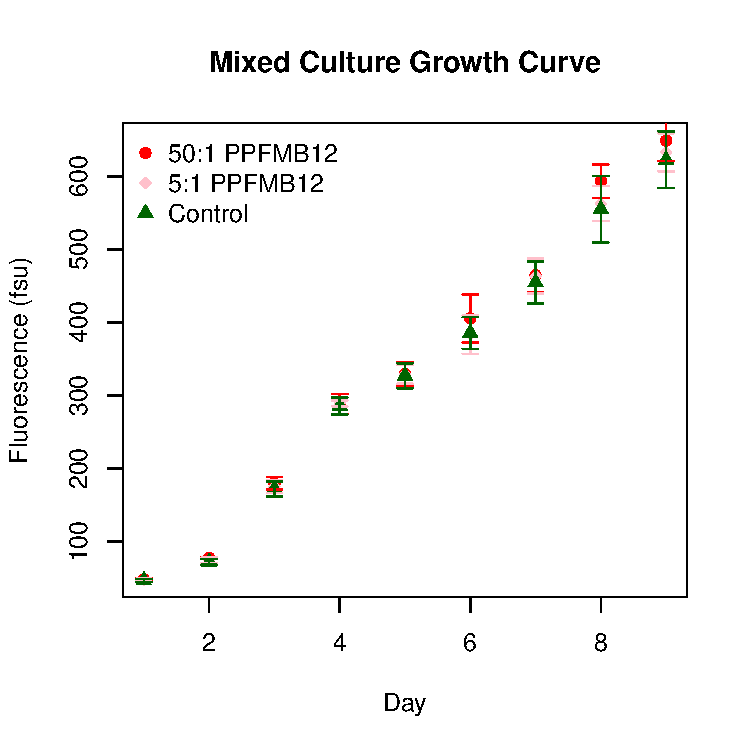
\includegraphics[width=1\textwidth]{./figure/ExpO_GrowthCurve1_unlabeled}
                                \end{figure}
                                \column{.5\textwidth}
                                \begin{figure}
                                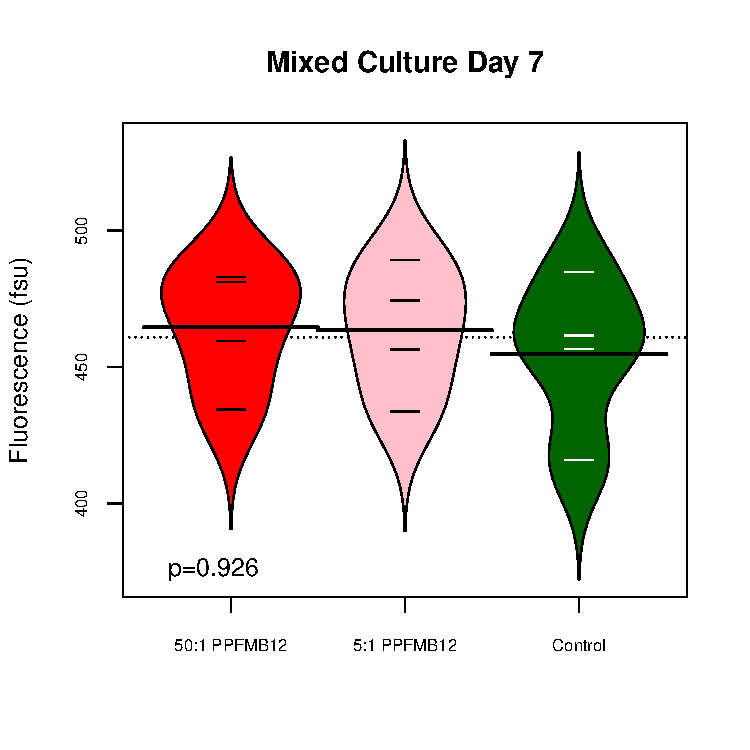
\includegraphics[width=1\textwidth]{./figure/ExpO_beanplot7_unlabeled}
                                \end{figure}
        \end{columns}
\end{frame}
%%%%%%%5
\section{B12 Assay}
\begin{frame}{Vitamin B12 Assay}
\begin{itemize}
\item Competitive ELISA assay test
\end{itemize}
%ExpF_AggregateData_1.tex
% latex table generated in R 3.1.1 by xtable 1.7-4 package
% Sun Nov  2 17:00:32 2014
\begin{table}[H]
\centering
\small{
\begin{tabular}{rlllrr}
  \hline
 & Species & Type & Processing & Avg. Conc. (ng/mL) &  St.Dev. (ng/mL) \\ 
  \hline
1 & Mixed Culture & Control & Homogenate & 0.29 & 0.25 \\ 
  2 & Mixed Culture & Control & Supernatant & 0.00 & 0.00 \\ 
  3 & Mixed Culture & Experimental & Homogenate & 0.06 & 0.11 \\ 
  4 & Mixed Culture & Experimental & Supernatant & 0.92 & 1.59 \\ 
  5 & Tetraselmis & Control & Homogenate & 0.14 & 0.12 \\ 
  6 & Tetraselmis & Control & Supernatant & 0.00 & 0.00 \\ 
  7 & Tetraselmis & Experimental & Homogenate & 0.28 & 0.47 \\ 
  8 & Tetraselmis & Experimental & Supernatant & 0.00 & 0.00 \\ 
   \hline
\end{tabular}
}
\caption{Adjusted algal data. Concentration in ng/mL, n=3.} 
\label{tab:AdjustedDataTable1}
\end{table}
%ExpF_PPFMrevised_2.tex
% latex table generated in R 3.1.1 by xtable 1.7-4 package
% Sun Nov  2 17:00:32 2014
\begin{table}[H]
\centering
\begin{tabular}{rllr}
  \hline
 & Material & Processing & Concentration (ng/mL) \\ 
  \hline
1 & F/2 media & NA & 1.79 \\ 
  2 & PPFM B12 & Supernatant & 39.37 \\ 
  3 & PPFM B12 & Homogenate & 41.19 \\ 
  4 & PPFM Broccoli & Supernatant & 44.93 \\ 
  5 & PPFM Broccoli & Homogenate & 45.87 \\ 
   \hline
\end{tabular}
\caption{Data for PPFM and F/2 media samples. Concentration in ng/mL, n=1.} 
\label{tab:PPFMrevised}
\end{table}


\end{frame}
%%%%%%%%%%%%
\section{Nutritional Analysis}
\begin{frame}{Nutritional Analysis}
\begin{itemize}
\item Analyze algal feedstock for lipid profile, amino acid content
\item Requires 2g dry algal biomass, 15L culture
\item Mixed algal culture \(\pm\) PPFM B12
\note[item]{selected algal/PPFM combination with potential for best results}
\note[item]{large volume culture, labor intensive set up and processing}
\end{itemize}
\begin{columns}[t] %Without t, the columns are centered
                \column{.5\textwidth}
                \begin{figure}
                                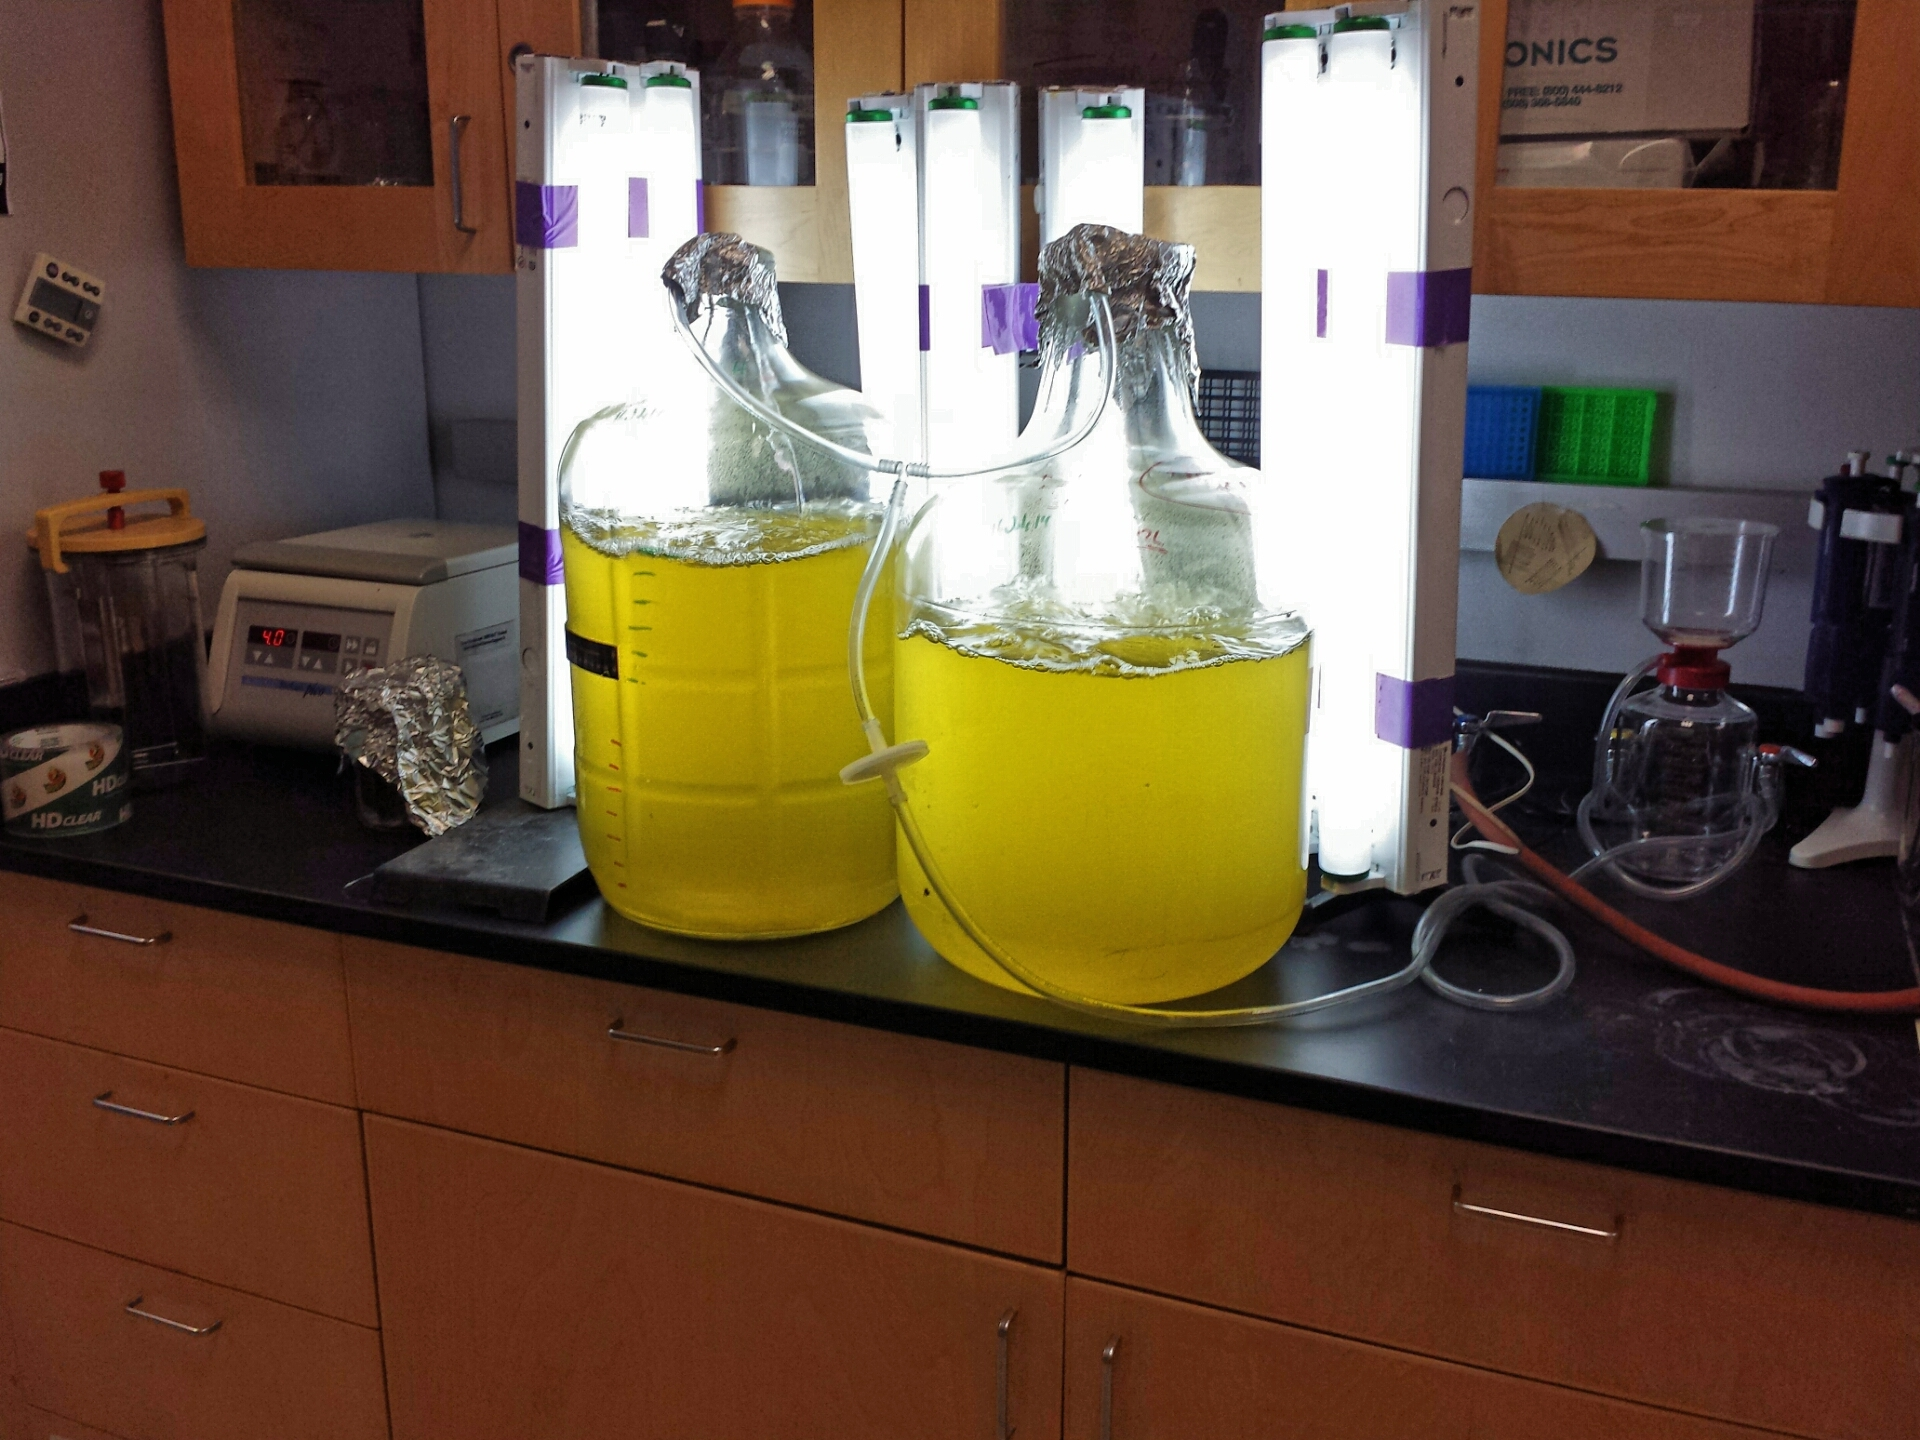
\includegraphics[width=1\textwidth]{./figure/large_vol_algae.jpg}
                                \end{figure}
                                \column{.5\textwidth}
                                \begin{figure}
                                \includegraphics[width=1\textwidth]{./figure/dried_algae.jpg}
                                \end{figure}
        \end{columns}


\end{frame}
%%%%%%%%%%%%%
\begin{frame}{Nutritional Analysis}


\begin{table}[ht]
\centering
\begin{tabular}{rlrrl}
  \hline
 & Compound & Algae Control & Algae + PPFM B12 & \% Change \\ 
  \hline
1 & Crude Protein & 21.80 & 29.46 & \textbf{\color{red}{35.14}} \\ 
  2 & Crude Fat & 9.07 & 19.58 & \textbf{\color{red}{115.88}} \\ 
   \hline
\end{tabular}
\caption{Summary of nutritional analysis results. Increased nutritional qualities are in red. Values represent grams per 100g of sample} 
\label{tab:MiscTable}
\end{table}


\end{frame}
%
%%%%%%%%%%%%%
\begin{frame}{Amino Acid Content}

% latex table generated in R 3.1.1 by xtable 1.7-4 package
% Sun Nov  2 15:43:11 2014
\begin{table}[ht]
\centering
{\small
\begin{tabular}{rlrrl}
  \hline
 & Compound & Algae Control & Algae + PPFM B12 & \% Change \\ 
  \hline
1 & Hydroxylysine & 0.15 & 0.43 & \textbf{\color{red}{186.67}} \\ 
  2 & Histidine & 0.33 & 0.60 & \textbf{\color{red}{81.82}} \\ 
  3 & Methionine & 0.39 & 0.68 & \textbf{\color{red}{74.36}} \\ 
  4 & Lysine & 0.79 & 1.26 & \textbf{\color{red}{59.49}} \\ 
  5 & Arginine & 0.93 & 1.44 & \textbf{\color{red}{54.84}} \\ 
  6 & Tyrosine & 0.59 & 0.89 & \textbf{\color{red}{50.85}} \\ 
  7 & Cysteine & 0.20 & 0.30 & \textbf{\color{red}{50.00}} \\ 
  8 & Leucine & 1.53 & 2.18 & \textbf{\color{red}{42.48}} \\ 
  9 & Proline & 0.93 & 1.30 & \textbf{\color{red}{39.78}} \\ 
  10 & Glycine & 1.09 & 1.52 & \textbf{\color{red}{39.45}} \\ 
  11 & Serine & 0.80 & 1.11 & \textbf{\color{red}{38.75}} \\ 
  12 & Glutamic Acid & 1.86 & 2.50 & \textbf{\color{red}{34.41}} \\ 
  13 & Phenylalanine & 1.02 & 1.37 & \textbf{\color{red}{34.31}} \\ 
  14 & Aspartic Acid & 1.79 & 2.40 & \textbf{\color{red}{34.08}} \\ 
  15 & Isoleucine & 0.86 & 1.15 & \textbf{\color{red}{33.72}} \\ 
  16 & Valine & 1.11 & 1.47 & \textbf{\color{red}{32.43}} \\ 
  17 & Threonine & 1.00 & 1.28 & \textbf{\color{red}{28.00}} \\ 
  18 & Alanine & 1.66 & 2.10 & \textbf{\color{red}{26.51}} \\ 
  19 & Hydroxyproline & 0.17 & 0.21 & \textbf{\color{red}{23.53}} \\ 
  20 & Tryptophan & 0.21 & 0.22 & \textbf{\color{red}{4.76}} \\ 
   \hline
\end{tabular}
}
\caption{Amino Acid profile for mixed algae culture nutritional analysis. Increased nutritional qualities are in red. Values represent grams per 100g of sample} 
\label{tab:AminoAcids_trim}
\end{table}

\end{frame}
%%%%%%
\begin{frame}{Fatty Acid Content}
% latex table generated in R 3.1.1 by xtable 1.7-4 package
% Sun Nov  2 15:43:11 2014
\begin{table}[ht]
\centering
{\small
\begin{tabular}{rlrrl}
  \hline
 & Compound & Algae Control & Algae + PPFM B12 & \% Change \\ 
  \hline
1 & DHA (22:6n3) & 3.19 & 5.04 & \textbf{\color{red}{57.99}} \\ 
  2 & Linolenic (18:3n3) & 5.14 & 7.61 & \textbf{\color{red}{48.05}} \\ 
  3 & Myristoleic (9c-14:1) & 0.23 & 0.30 & \textbf{\color{red}{30.43}} \\ 
  4 & Myristic (14:0) & 7.67 & 9.47 & \textbf{\color{red}{23.47}} \\ 
  5 & Linoleic (18:2n6) & 3.37 & 4.14 & \textbf{\color{red}{22.85}} \\ 
  6 & Behenoic (22:0) & 0.54 & 0.63 & \textbf{\color{red}{16.67}} \\ 
  7 & 10c-17:1 & 1.53 & 1.60 & \textbf{\color{red}{4.58}} \\ 
  8 & Oleic (9c-18:1) & 19.34 & 19.15 & \textbf{\color{blue}{-0.98}} \\ 
  9 & Lignoceric (24:0) & 0.16 & 0.14 & \textbf{\color{blue}{-12.50}} \\ 
  10 & EPA (20:5n3) & 4.58 & 3.93 & \textbf{\color{blue}{-14.19}} \\ 
  11 & Stearic (18:0) & 0.46 & 0.39 & \textbf{\color{blue}{-15.22}} \\ 
  12 & C15:0 & 0.42 & 0.34 & \textbf{\color{blue}{-19.05}} \\ 
  13 & C16:0 [Palmitic] & 24.19 & 19.58 & \textbf{\color{blue}{-19.06}} \\ 
  14 & Palmitoleic (9c-16:1) & 15.25 & 11.95 & \textbf{\color{blue}{-21.64}} \\ 
  15 & Margaric (17:0) & 0.33 & 0.21 & \textbf{\color{blue}{-36.36}} \\ 
   \hline
\end{tabular}
}
\caption{Fatty Acid profile for mixed algae culture nutritional analysis. Increased nutritional qualities are in red. Values represent grams per 100g of sample} 
\label{tab:FattyAcids_trim}
\end{table}

\end{frame}
%%%%%
%
\section{Conclusions}
\begin{frame}{Conclusions \& Future Directions}
\begin{itemize}
\item PPFM species identified
\item Potential increase in nutritional qualities independent of growth rate
\end{itemize}

\begin{figure}
                                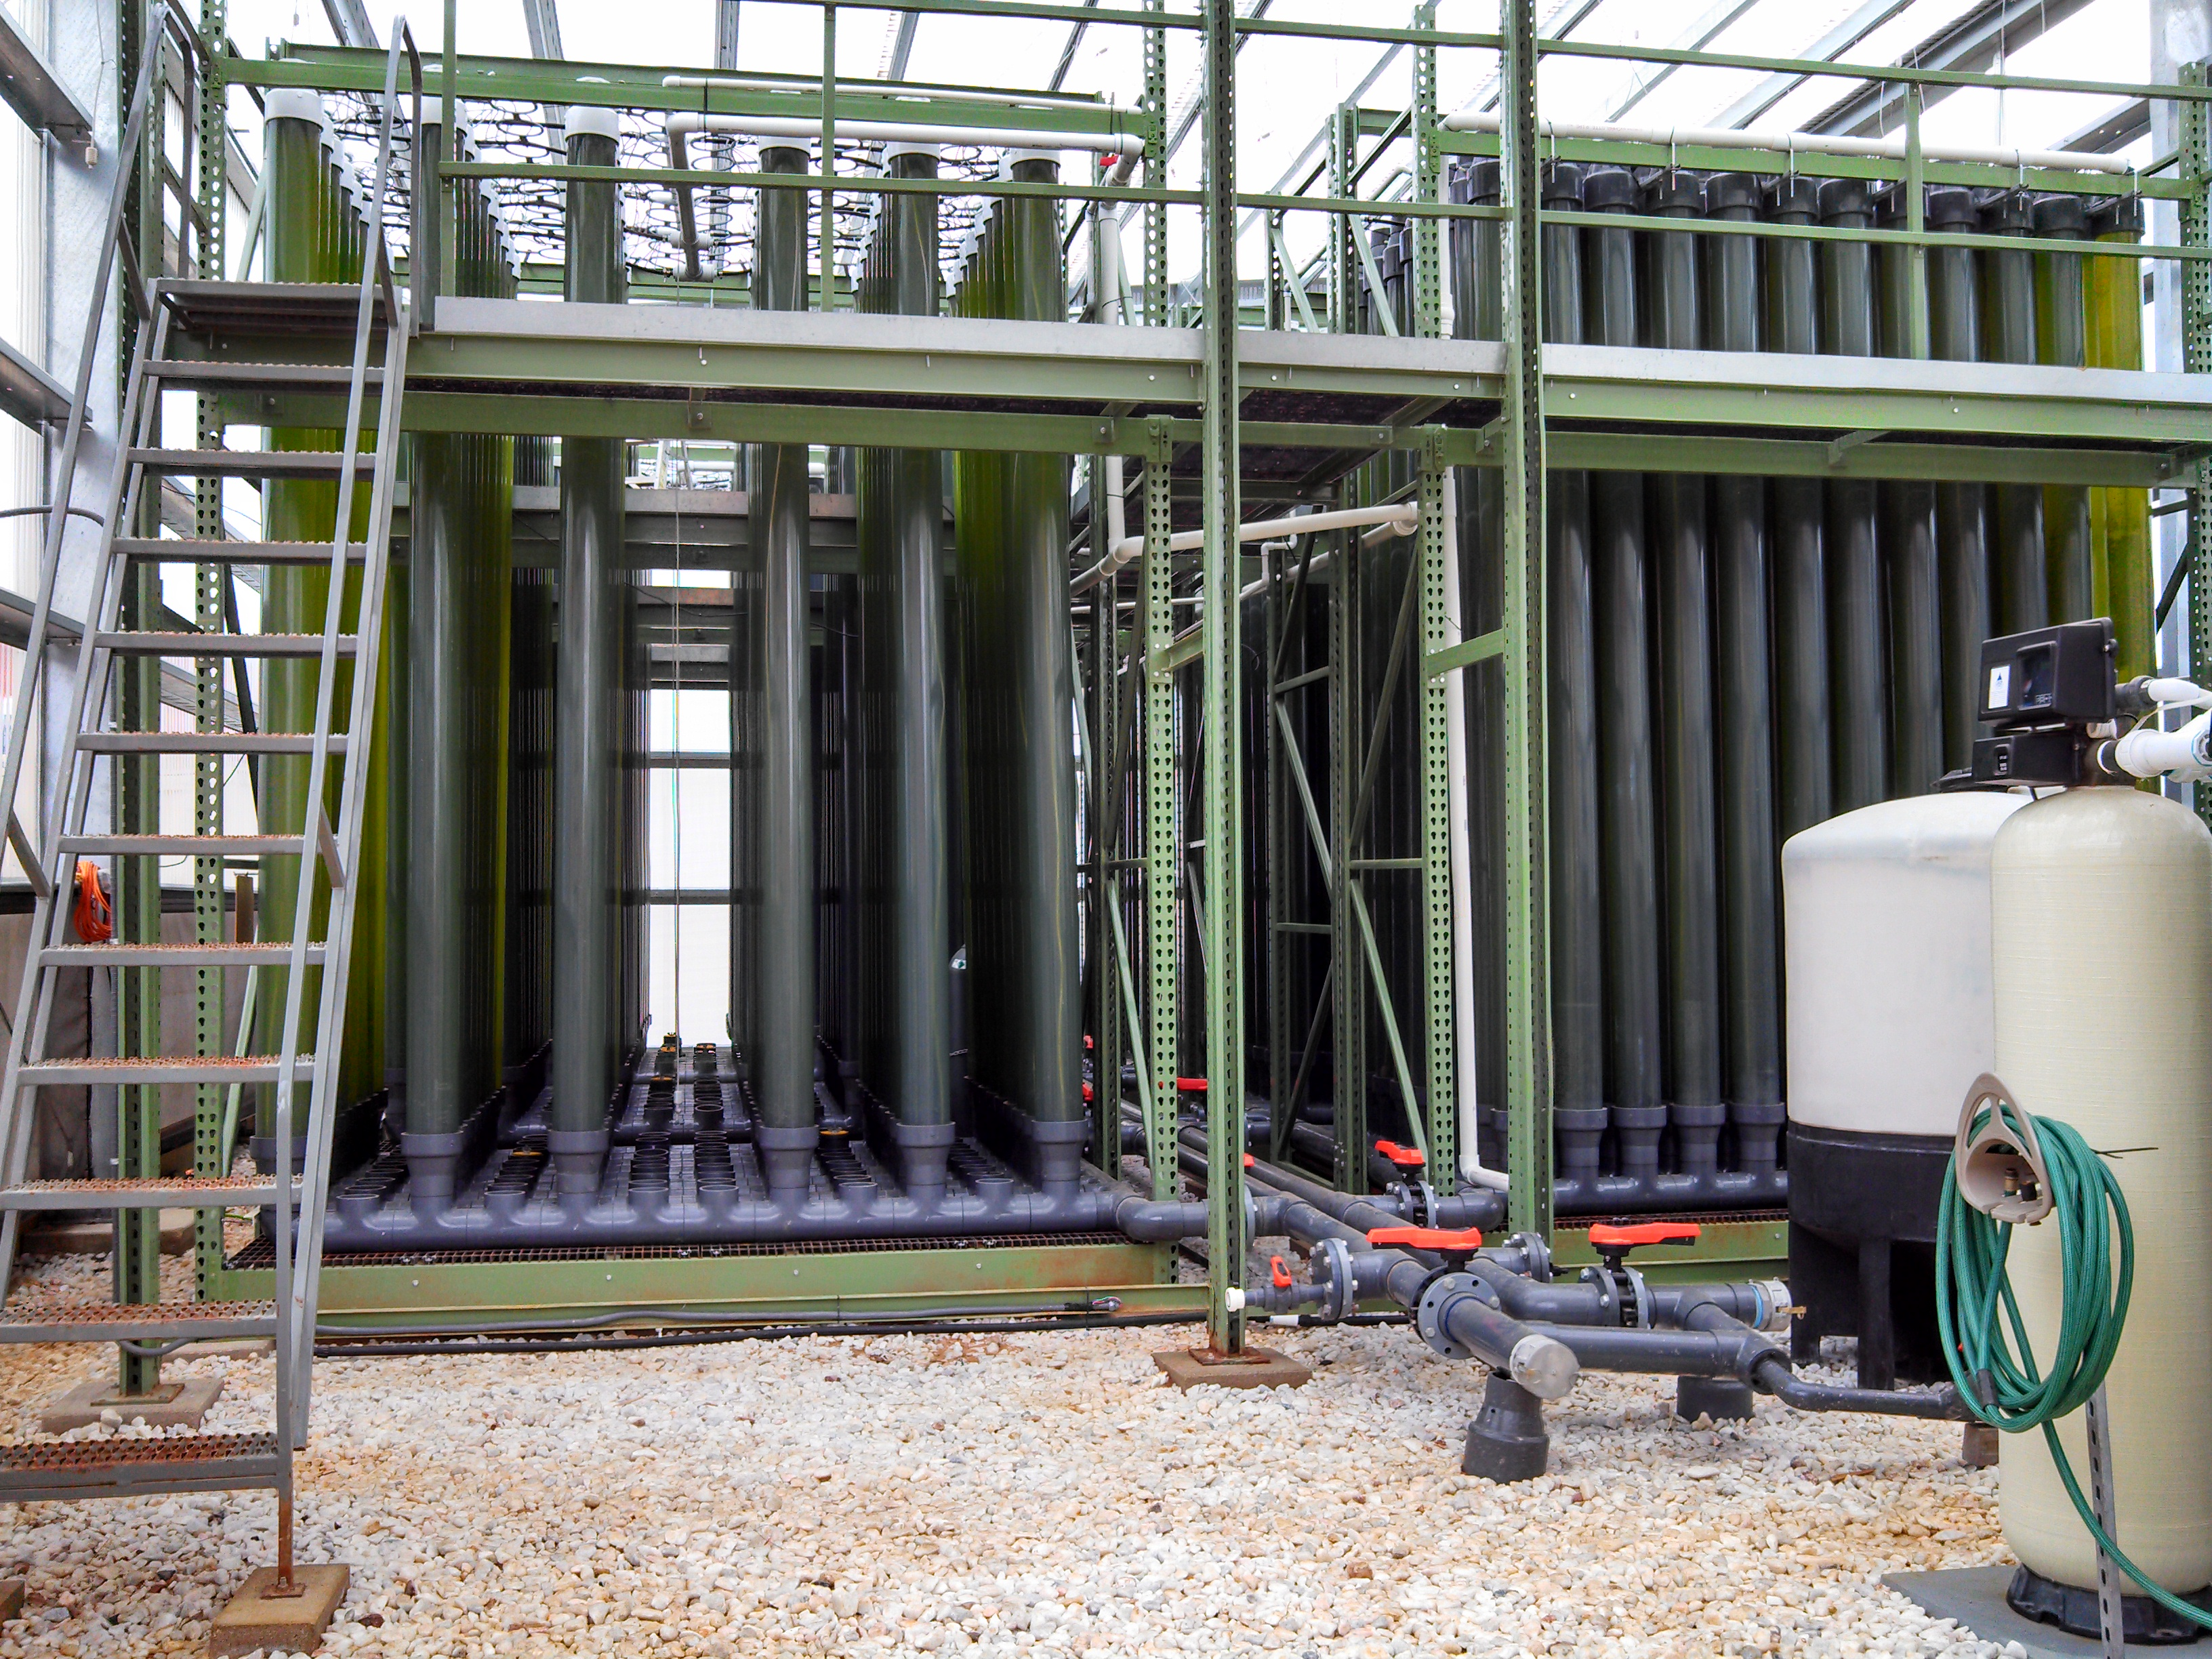
\includegraphics[width=0.7\textwidth]{./figure/UTEXAlgalBioreactors.jpg}
                                \caption{Algal bioreactors, Austin, TX}
                                \end{figure}

\end{frame}
%
% \section{End}
\begin{frame}{Acknowledgements}
\begin{itemize}
\item Acknowledgements
  \begin{itemize}
  \item Graduate Committee members
  \item SU Biology Department faculty
  \item TEDCO funding 
  \item RAP funding
  \item Horn Point Laboratories
  \item UTEX Algae Culture Collection
  \end{itemize}
  \begin{figure}

\includegraphics[width=0.5\textwidth]{./figure/bigSU.PNG}
\end{figure}
\end{itemize}
\begin{figure}[hb!]
    \centering
    
\includegraphics[scale=0.25]{./figure/tedco_logo_tedco_md}%[width=0.3\textwidth]
    \caption{Technology \& Economic Development Corporation of Maryland, Technology Validation Program}
\end{figure}
% \bibliography{MyLibrary.bib}
% \bibliographystyle{NAR}
\end{frame}
%
%%%%%%%%%%%%%%%%%%%
% \section{sample}
% \begin{frame}{sample}
% \begin{itemize}
%   \item
%   \end{itemize}
% \end{frame}
% \begin{figure}
%     \centering
%     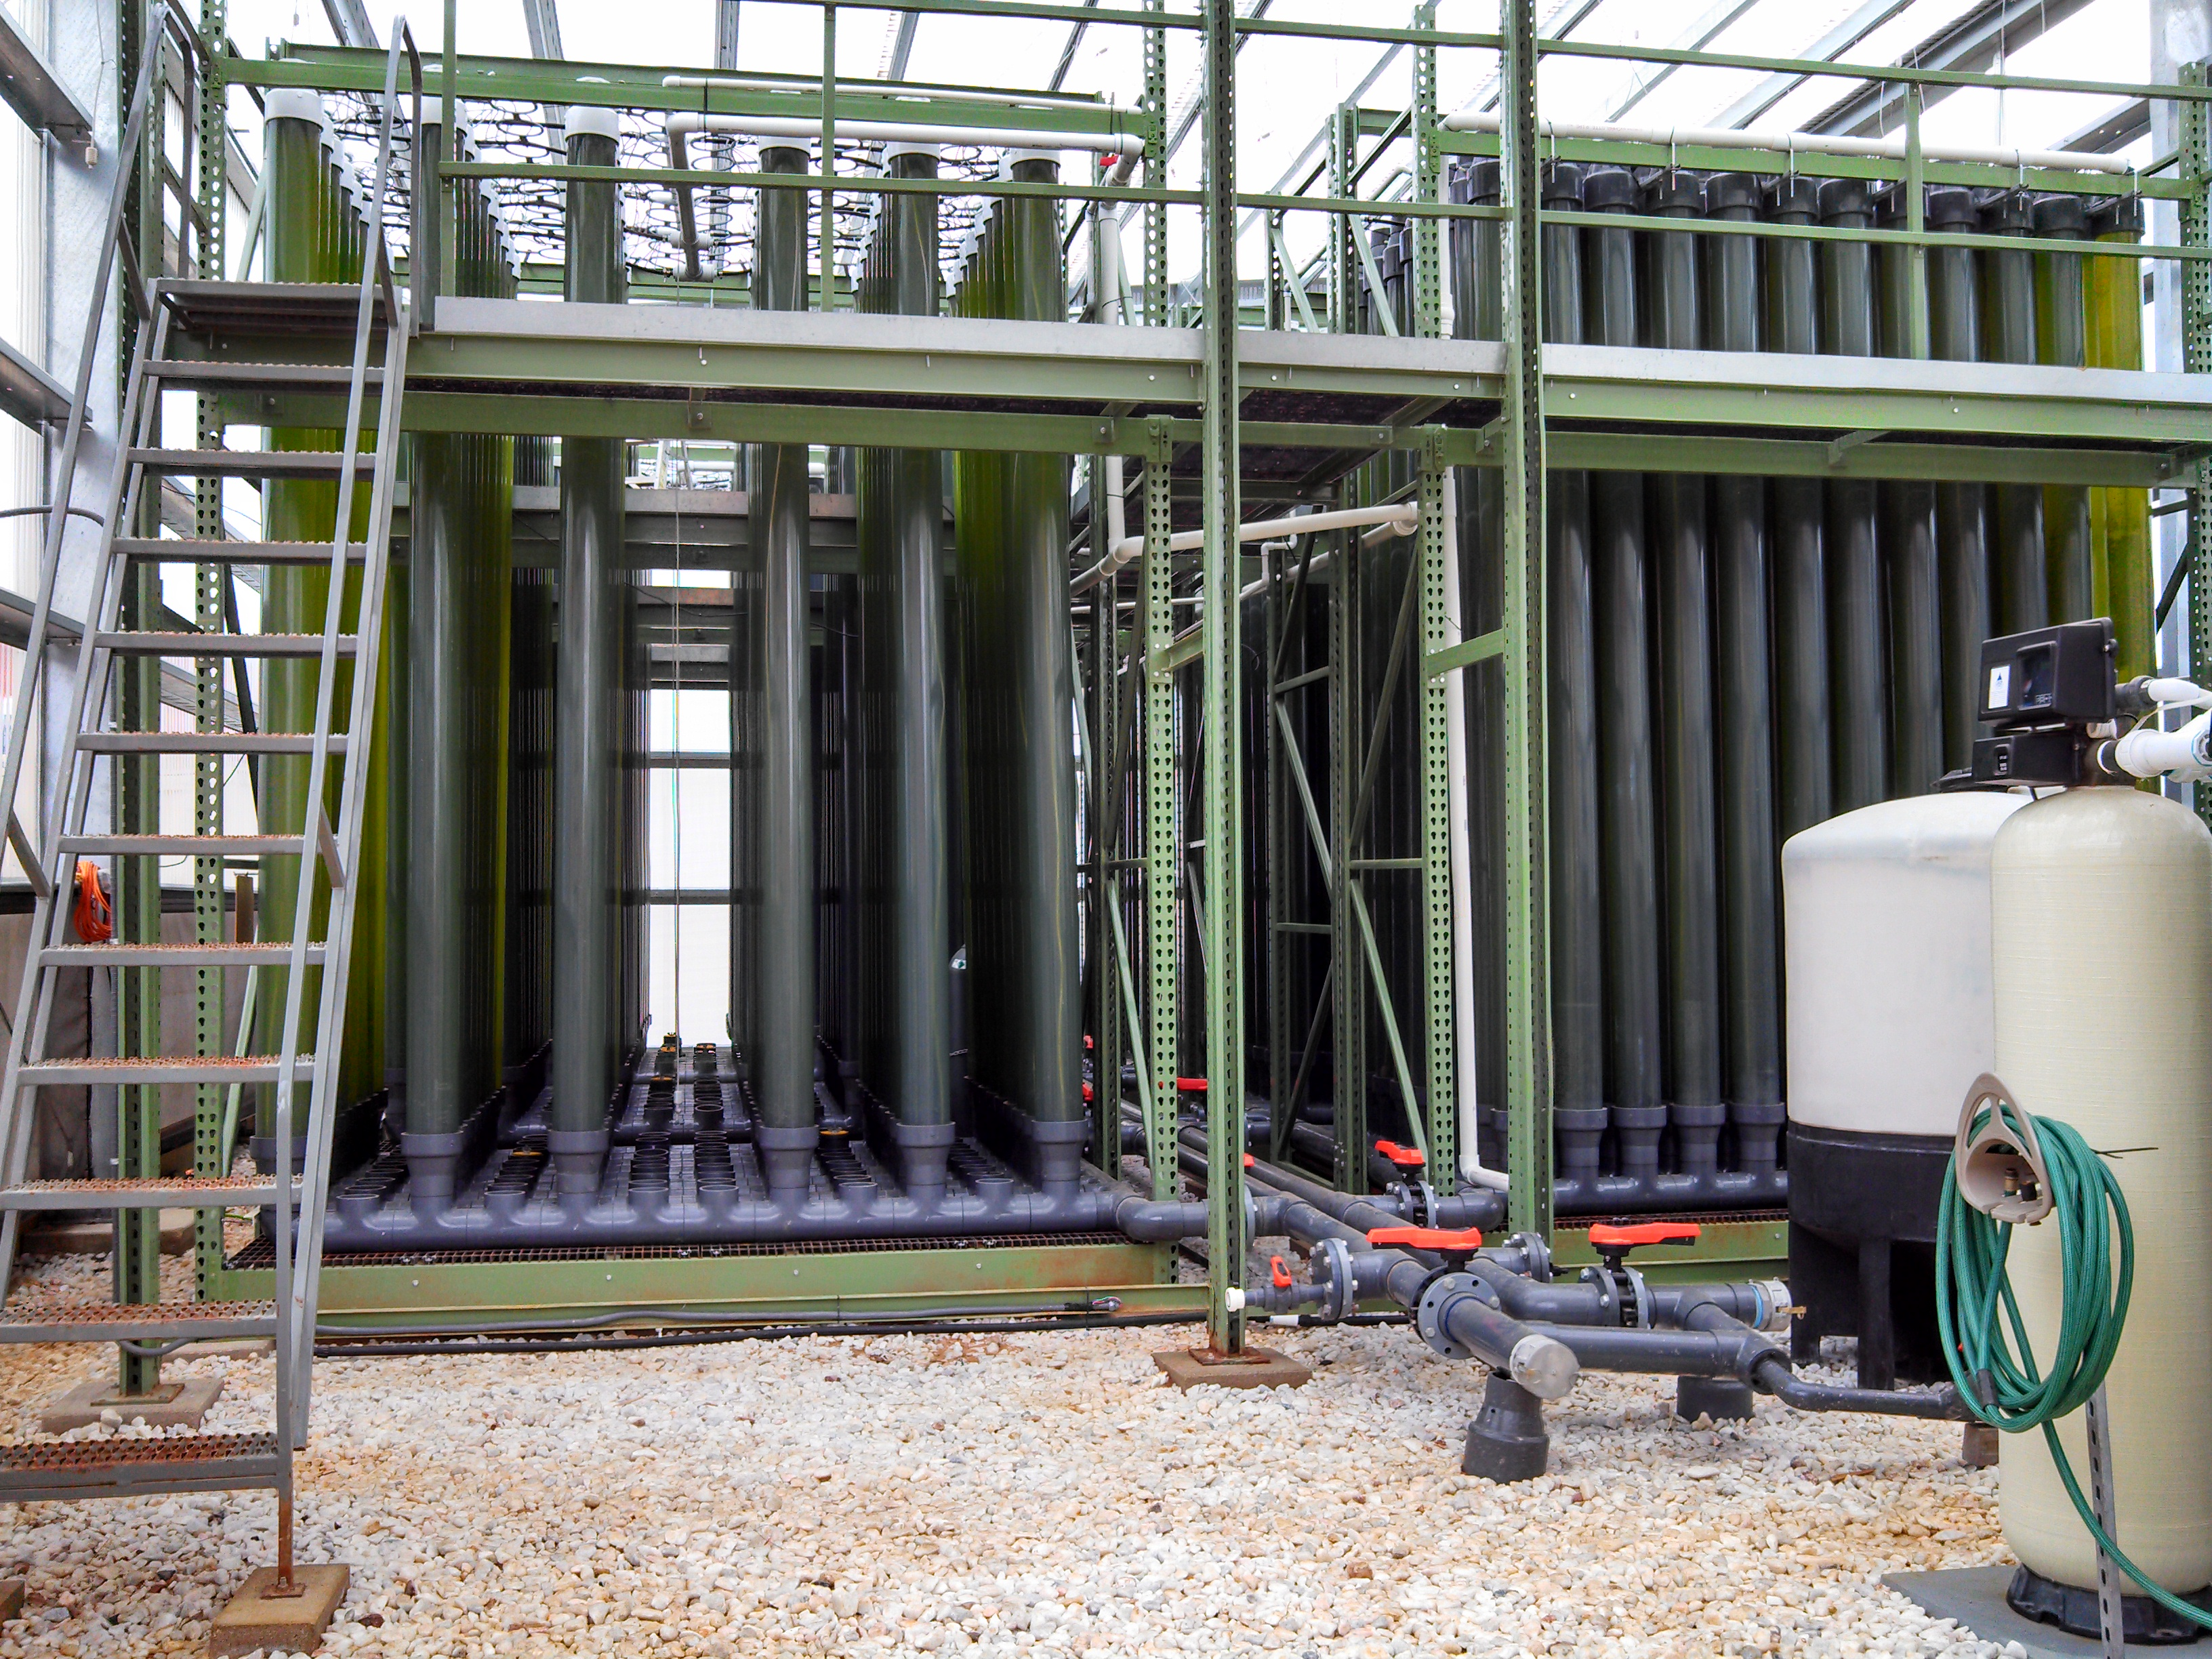
\includegraphics[width=0.2\textwidth]{./figure/UTEXAlgalBioreactors.jpg}
%     \caption{Algal bioreactors, Austin, TX}
%     \label{}
% \end{figure}
% 
% \begin{figure}
%     \centering
%     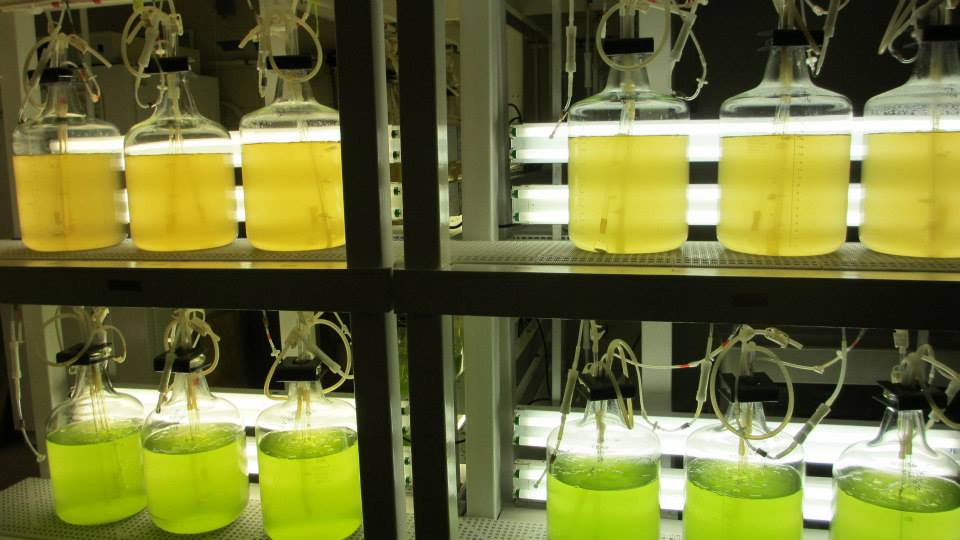
\includegraphics[width=0.2\textwidth]{./figure/HPL_Experiment_underway.jpg}
%     \caption{Algae grown for aquaculture. Source: Horn Point Laboratory}
%     \label{}
% \end{figure}
% \includegraphics[scale=1][width=1\textwidth]{./figure/FAO_Isochrysis_Tetraselmis.jpg}

\end{document}
